\documentclass[11pt,a4paper]{article}
\usepackage[T1]{fontenc}
\usepackage[utf8]{inputenc}
\usepackage{lmodern}
\usepackage[margin=22mm,headheight=16pt]{geometry}
\usepackage{amsmath,amssymb,graphicx,array,longtable,booktabs}
\usepackage{microtype,xcolor,hyperref,xurl,fancyhdr}
\definecolor{Navy}{HTML}{17324D}
\definecolor{Teal}{HTML}{087F8C}
\definecolor{Gold}{HTML}{B88128}
\hypersetup{colorlinks=true,linkcolor=Navy,urlcolor=Teal,bookmarksnumbered=true,hypertexnames=false}
\setlength{\parindent}{0pt}
\setlength{\parskip}{6pt}
\setlength{\emergencystretch}{4em}
\setcounter{tocdepth}{1}
\pagestyle{fancy}\fancyhf{}
\fancyfoot[R]{\small\thepage}
\fancyfoot[L]{\small\sffamily Sharif University of Technology}
\renewcommand{\headrulewidth}{0.3pt}
\makeatletter
\renewcommand\section{\@startsection{section}{1}{\z@}{-3.2ex plus -1ex minus -.2ex}{1.6ex plus .2ex}{\normalfont\Large\sffamily\bfseries\color{Navy}}}
\renewcommand\subsection{\@startsection{subsection}{2}{\z@}{-2.5ex plus -1ex minus -.2ex}{1.2ex plus .2ex}{\normalfont\large\sffamily\bfseries\color{Teal}}}
\makeatother
\fancyhead[L]{\small\sffamily\color{Navy}Reza Sanaee Nezhad}\fancyhead[R]{\small\sffamily\color{Teal}Technical Report}\begin{document}
\begin{titlepage}\centering\vspace*{7mm}

\includegraphics[width=31mm]{assets/sharif_emblem_en.png}\par\vspace{5mm}
{\Large\sffamily\bfseries\color{Navy}SHARIF UNIVERSITY OF TECHNOLOGY\par}
\vspace{2mm}{\sffamily Department of Electrical Engineering\par}
\vspace{17mm}{\color{Teal}\rule{\linewidth}{1.4pt}}\par\vspace{6mm}
{\large\sffamily\color{Teal}TECHNICAL REPORT\par}
\vspace{8mm}{\huge\sffamily\bfseries\color{Navy}RDD Streaming, Cardinality Sketches, and PageRank Algorithms\par}
\vspace{9mm}{\color{Gold}\rule{45mm}{1pt}}\par\vfill
\begin{minipage}{.88\linewidth}{\sffamily\color{Teal}AUTHOR}\par{\Large\sffamily Reza Sanaee Nezhad}\par Student ID: 401101502\par\vspace{7mm}
{\sffamily\color{Teal}INSTRUCTOR / INSTRUCTORS}\par
Dr Iman Gholampour\par\vspace{7mm}
{\sffamily\color{Teal}ACADEMIC CONTEXT}\par
Big Data Processing\par\end{minipage}\vfill
\end{titlepage}
\tableofcontents\clearpage
\section{Theory 1: graph model and transition convention}

The graph has A -> B,C,D;\allowbreak{} B -> A,D;\allowbreak{} C -> A;\allowbreak{} D -> B,C. With destination rows and source columns in order A,B,C,D, the column-stochastic matrix is:\allowbreak{}


\begingroup\small\setlength{\tabcolsep}{3pt}\renewcommand{\arraystretch}{1.2}
\begin{longtable}{@{}p{0.1760\linewidth}p{0.1760\linewidth}p{0.1760\linewidth}p{0.1760\linewidth}p{0.1760\linewidth}@{}}
\toprule
\textbf{Destination/\allowbreak{}source} & \textbf{A} & \textbf{B} & \textbf{C} & \textbf{D} \\ \midrule
\endfirsthead
\textbf{Destination/\allowbreak{}source} & \textbf{A} & \textbf{B} & \textbf{C} & \textbf{D} \\ \midrule \endhead
A & 0 & 1/\allowbreak{}2 & 1 & 0 \\
B & 1/\allowbreak{}3 & 0 & 0 & 1/\allowbreak{}2 \\
C & 1/\allowbreak{}3 & 0 & 0 & 1/\allowbreak{}2 \\
D & 1/\allowbreak{}3 & 1/\allowbreak{}2 & 0 & 0 \\
\bottomrule\end{longtable}\endgroup

Solve r=\allowbreak{}0.85 M r+\allowbreak{}0.15 e with the appropriate normalized teleport distribution. B/\allowbreak{}C/\allowbreak{}D have equal stationary scores in some of these teleport configurations despite having different outgoing-link structures. The stationary numerical vectors are provided in the numerical calculations section below. Focused teleport favors its seed directly and influences other nodes through the actual graph transitions. TrustRank uses e=\allowbreak{}(0,1,0,0). Raw spam mass is 1-TR/\allowbreak{}PR and can be negative for trusted pages. Clipping negative values to zero is an optional display convention and must be stated. HITS authority and hub vectors are eigenvectors associated with incoming/\allowbreak{}outgoing good-link structure and depend on normalization. PageRank describes a different random-walk model;\allowbreak{} their orderings need not agree.

\[ r_{t+1}(v)=\frac{1-\beta}{N}+\frac{\beta d_t}{N}+\beta\sum_u r_t(u)P(u\to v). \]
\section{Theory 2: complete DGIM bucket trace}

Process the sixteen-bit sequence in timestamp order, storing at most two buckets per power-of-two size and merging the two oldest equal-size buckets. A bucket timestamp is its newest represented one, not the start of its interval. At t=\allowbreak{}12 the buckets newest-first are (1,12),(2,11),(2,8),(4,5). At t=\allowbreak{}13 add (1,13), leaving two unit buckets. t=\allowbreak{}14 is zero. At t=\allowbreak{}15 add (1,15);\allowbreak{} merge the older unit buckets into (2,13), then merge the older size-two buckets into (4,11). At t=\allowbreak{}16 add (1,16).


\begingroup\small\setlength{\tabcolsep}{3pt}\renewcommand{\arraystretch}{1.2}
\begin{longtable}{@{}p{0.3100\linewidth}p{0.3100\linewidth}p{0.3100\linewidth}@{}}
\toprule
\textbf{Final bucket size} & \textbf{Timestamp} & \textbf{Represented one timestamps} \\ \midrule
\endfirsthead
\textbf{Final bucket size} & \textbf{Timestamp} & \textbf{Represented one timestamps} \\ \midrule \endhead
1 & 16 & 16 \\
1 & 15 & 15 \\
2 & 13 & 12,13 \\
4 & 11 & 7,8,10,11 \\
4 & 5 & 1,3,4,5 \\
\bottomrule\end{longtable}\endgroup

For N=\allowbreak{}12, timestamp 5 is still allowed at t=\allowbreak{}16, although that oldest bucket includes earlier ones. For K=\allowbreak{}7 the query covers t=\allowbreak{}10..16. Sum the fully included newest buckets and half the boundary bucket:\allowbreak{} 1+\allowbreak{}1+\allowbreak{}2+\allowbreak{}4/\allowbreak{}2=\allowbreak{}6. The exact last-seven count is also six, giving absolute error zero and relative error zero. Exact agreement in this example does not make DGIM an exact counter in general.

\begingroup\small\setlength{\tabcolsep}{3pt}\renewcommand{\arraystretch}{1.18}\begin{longtable}{@{}p{0.2200\linewidth}p{0.2200\linewidth}p{0.2200\linewidth}p{0.2200\linewidth}@{}}
\caption{Theory 2: complete DGIM bucket trace - numerical data and parameters.}\label{tab:036_p006_table10}\\\toprule
\textbf{Bucket} & \textbf{Size} & \textbf{Timestamp} & \textbf{Represented one timestamps} \\ \midrule\endfirsthead \textbf{Bucket} & \textbf{Size} & \textbf{Timestamp} & \textbf{Represented one timestamps} \\ \midrule\endhead
1 & 1 & 16 & 16 \\
2 & 1 & 15 & 15 \\
3 & 2 & 13 & 12, 13 \\
4 & 4 & 11 & 7, 8, 10, 11 \\
5 & 4 & 5 & 1, 3, 4, 5 \\
\bottomrule\end{longtable}\endgroup
\clearpage
\section{Theory 3: FM maximum register}

The six hash strings have trailing-zero counts 3,5,4,3,3,6;\allowbreak{} R=\allowbreak{}6 and the simple estimate is 64. A nine-bit all-zero string gives a capped trailing-zero count of 9 and estimate 512 under the exercise convention. A finite-width implementation must explicitly handle zero hashes instead of looping indefinitely. One unusually long zero suffix can double the estimate for every additional register bit. Therefore the estimate can overshoot or undershoot the true count, and adding one element need not reduce error. Uniform hashes give a suffix probability of about 2\textasciicircum{}(-k), explaining the noisy maximum statistic.

\section{Theory 4: Bloom-filter derivation}

Each partition has n/\allowbreak{}k bits and receives one hash per inserted element. A selected bit remains zero with probability (1-k/\allowbreak{}n)\textasciicircum{}m, approximately exp(-mk/\allowbreak{}n). Under independent partitions, false-positive probability is [1-(1-k/\allowbreak{}n)\textasciicircum{}m]\textasciicircum{}k, approximately (1-exp(-mk/\allowbreak{}n))\textasciicircum{}k. A conventional single-array filter has a closely related approximation, not an exactly identical finite-size occupancy model. Minimize the log of the approximation in continuous k to obtain k=\allowbreak{}(n/\allowbreak{}m) ln 2;\allowbreak{} choose a nearby positive integer and require valid partition sizes. Independence and uniformity are modeling assumptions.

\section{Theory 5: cooperating spam farms}

The submission proposes mutual target-page links while support pages point to their own target. A mutual link can retain or redirect some probability within the combined farm. However each new outgoing link also divides the source target's outgoing probability, and benefits depend on support links, external inflow, and the recorded farm model. Without those constraints, the proposed connection is a candidate strategy, not a proved universal PageRank-maximizing topology.

\section{Practical 1: file-based stream simulation}

A Python feeder reads traffic.csv in chunks of 5000 records and publishes a new CSV file every five seconds. Spark's textFileStream watches the input directory and detects newly created files. Files should be written completely and atomically renamed into the watched directory so that a partial file is not consumed. Replaying a static dataset creates a simulated arrival stream, not live camera telemetry. The StreamingContext uses a five-second batch interval. Parsing extracts camera from index 0, passage time from index 4, and plate from index 6. Console samples demonstrate newly arriving tuples in successive batches. Splitting on commas assumes simple unquoted fields;\allowbreak{} a CSV-aware parser is needed when fields may contain quoted commas. The screenshots document this classroom run without establishing exactly-once delivery or restart recovery.

\begin{figure}[!htbp]\centering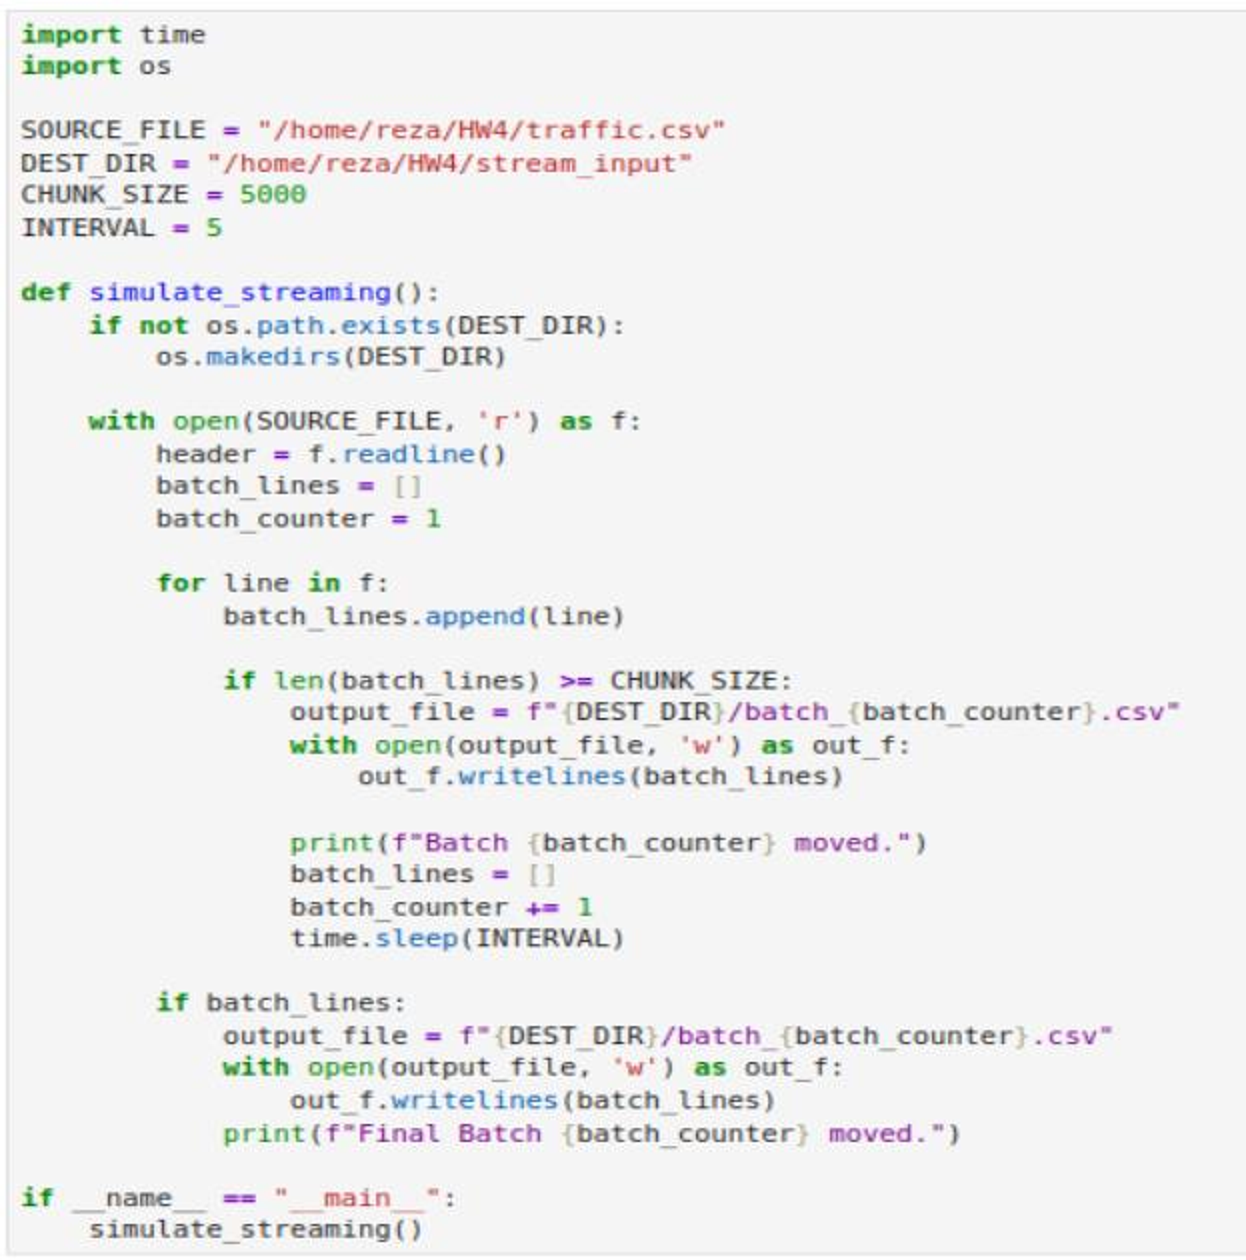
\includegraphics[width=\linewidth,height=.72\textheight,keepaspectratio]{assets/036_p013_03.png}\caption{Implementation and output: Practical 1: file-based stream simulation.}\label{fig:036_p013_030}\end{figure}
\begin{figure}[!htbp]\centering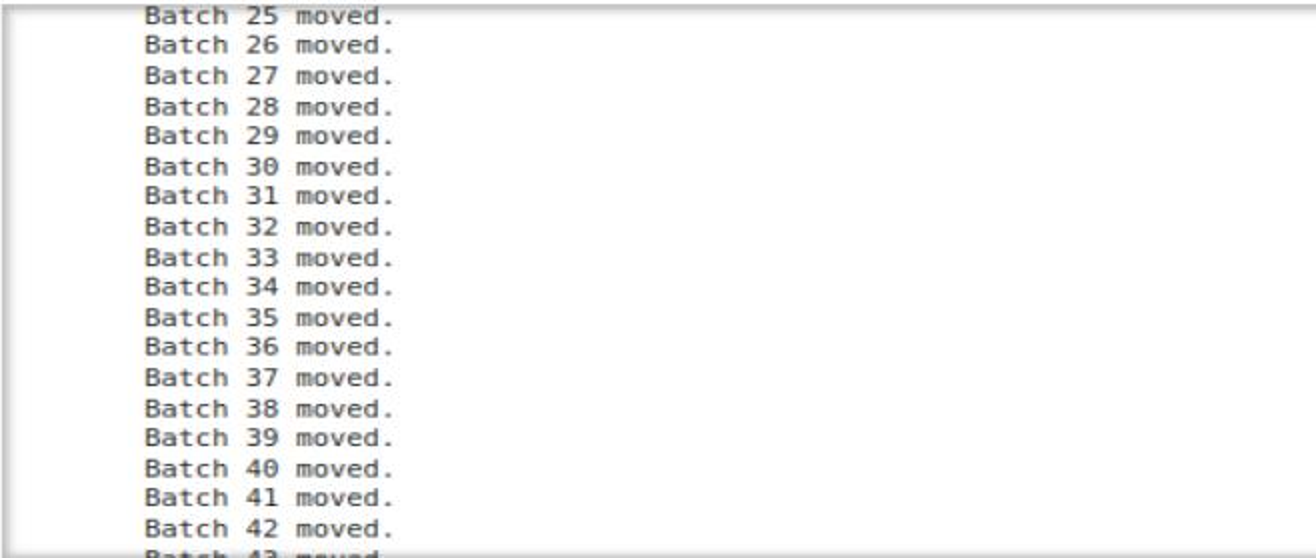
\includegraphics[width=\linewidth,height=.72\textheight,keepaspectratio]{assets/036_p014_01.png}\caption{Diagram or recorded result: Practical 1: file-based stream simulation.}\label{fig:036_p014_010}\end{figure}
\begin{figure}[!htbp]\centering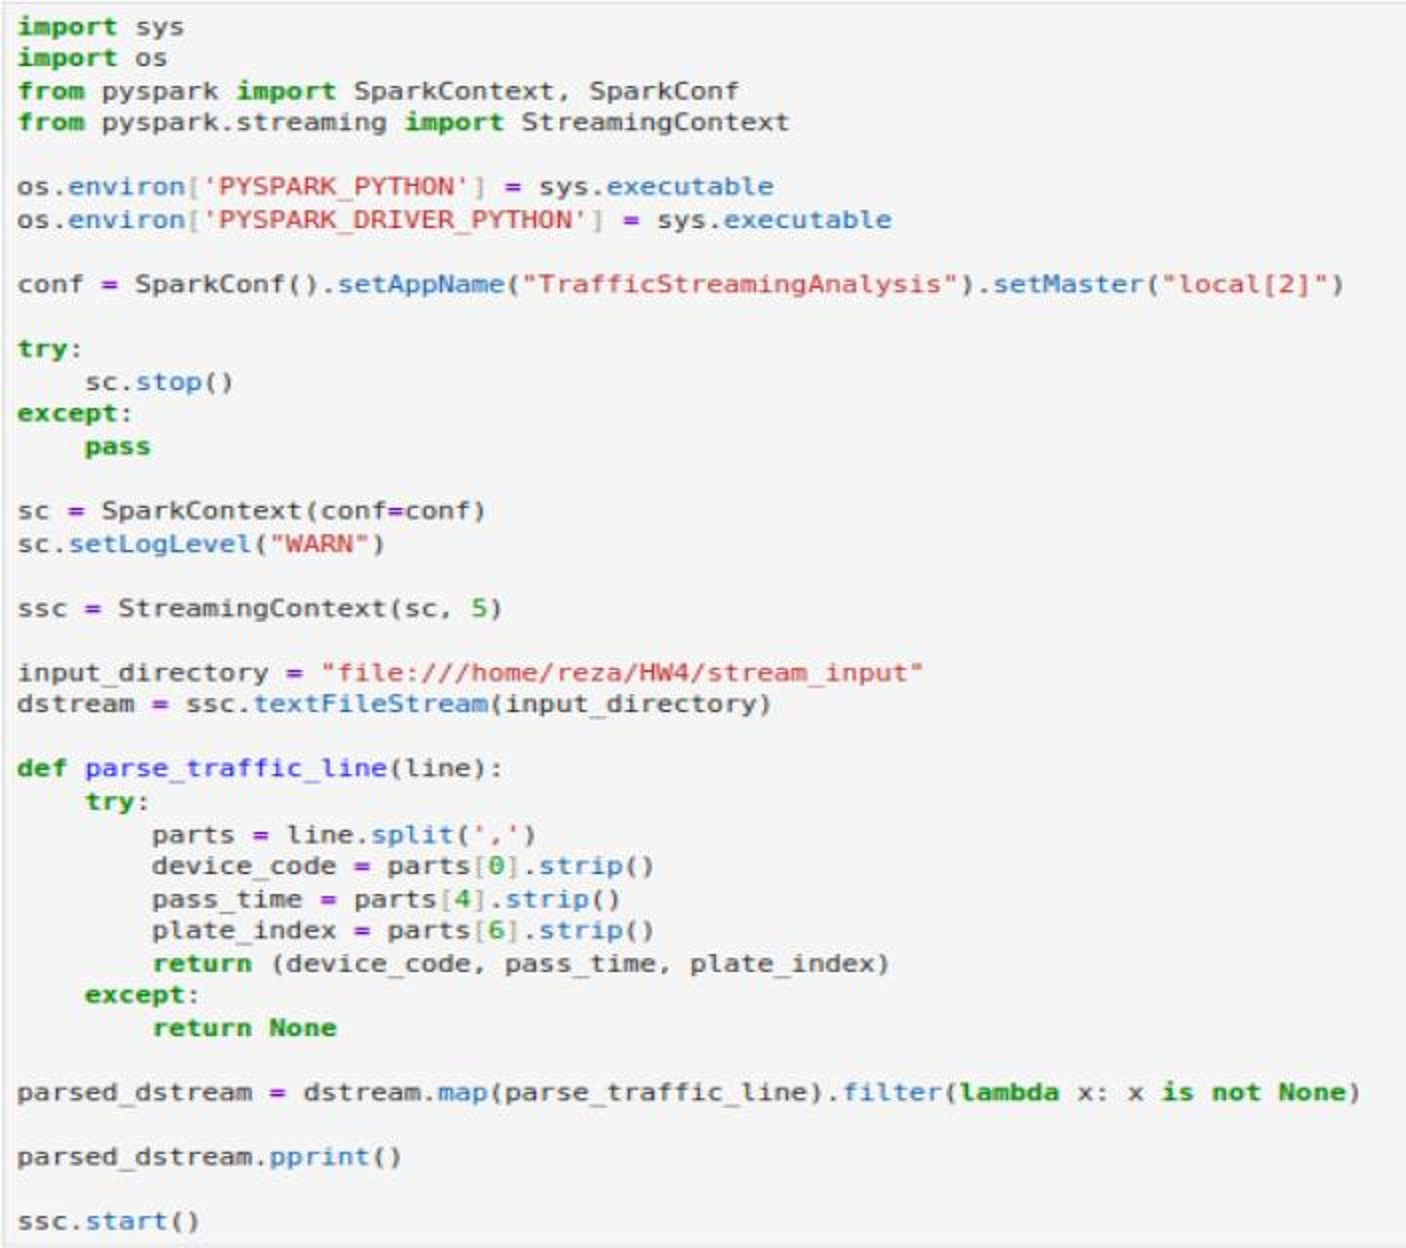
\includegraphics[width=\linewidth,height=.72\textheight,keepaspectratio]{assets/036_p014_02.png}\caption{Implementation and output: Practical 1: file-based stream simulation.}\label{fig:036_p014_020}\end{figure}
\begin{figure}[!htbp]\centering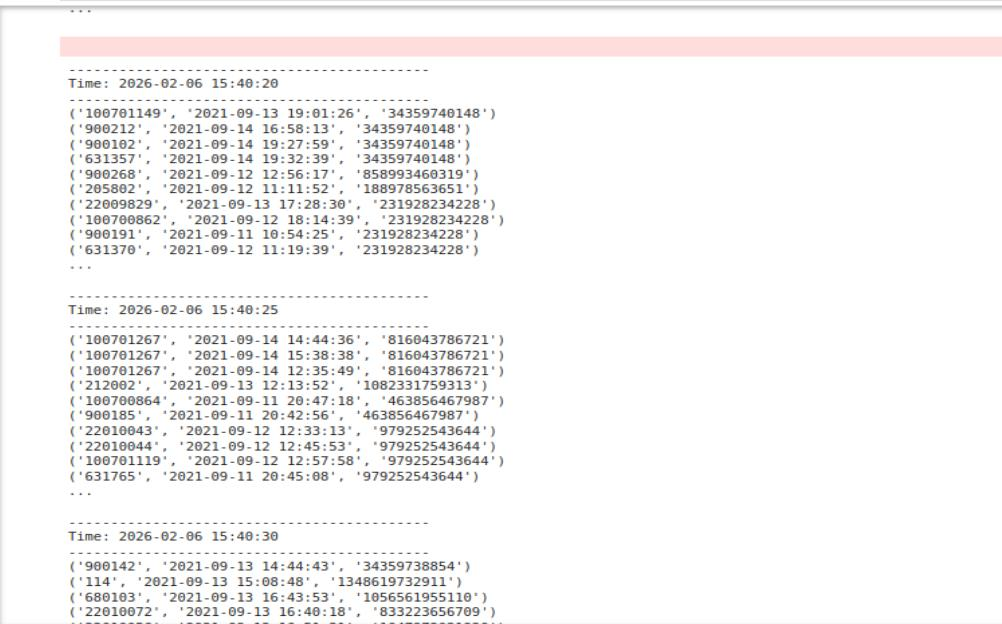
\includegraphics[width=\linewidth,height=.72\textheight,keepaspectratio]{assets/036_p015_01.png}\caption{Diagram or recorded result: Practical 1: file-based stream simulation.}\label{fig:036_p015_010}\end{figure}
\clearpage
\section{Volume windows and top-three cameras}

A thirty-second window advances every ten seconds, covering six five-second batches when full. At the configured feeder rate, a full window can contain about 30000 records. Early counts rise while the window fills;\allowbreak{} later counts reflect replay-arrival time, not necessarily a real thirty-second interval in the recorded timestamps. reduceByKey obtains counts by camera, and sorting selects the top three. The submitted examples repeatedly identify cameras 900212 and 100700853 among high-count cameras, with sample counts rising from about 200 toward 400 as the window fills. These counts should not be presented as a measured physical camera flow rate because the feeder compresses/\allowbreak{}replays the data. A larger window smooths fluctuations but retains older arrivals;\allowbreak{} a smaller window reacts faster but is noisier. A thirty-second window does not guarantee a thirty-second maximum detection delay because triggers, backlog, and processing also contribute. Ranking agreement with an earlier static analysis is a consistency observation, not an independent correctness proof.

\begin{figure}[!htbp]\centering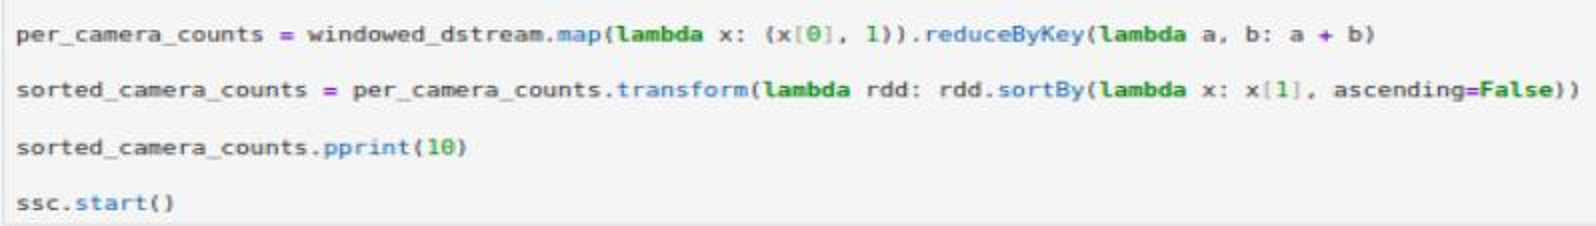
\includegraphics[width=\linewidth,height=.72\textheight,keepaspectratio]{assets/036_p016_02.png}\caption{Implementation and output: Volume windows and top-three cameras.}\label{fig:036_p016_020}\end{figure}
\begin{figure}[!htbp]\centering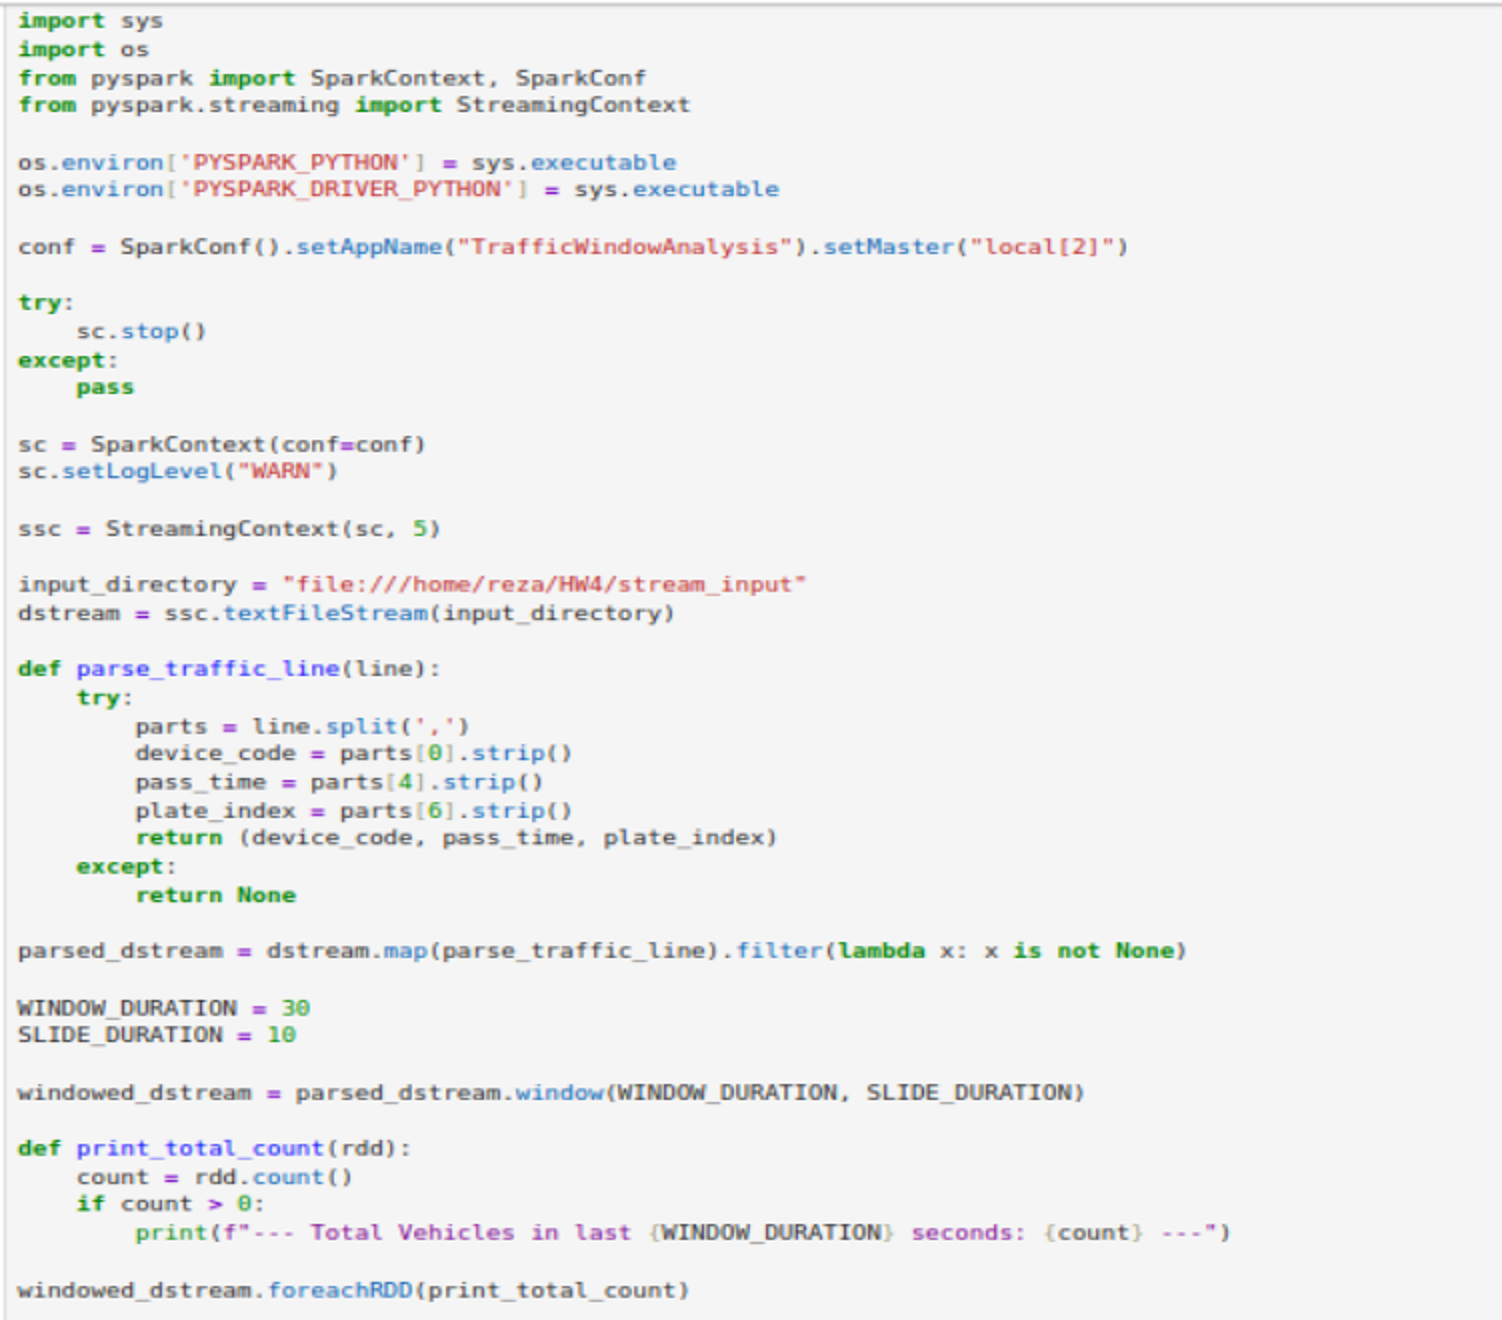
\includegraphics[width=\linewidth,height=.72\textheight,keepaspectratio]{assets/036_p016_03.png}\caption{Implementation and output: Volume windows and top-three cameras.}\label{fig:036_p016_030}\end{figure}
\begin{figure}[!htbp]\centering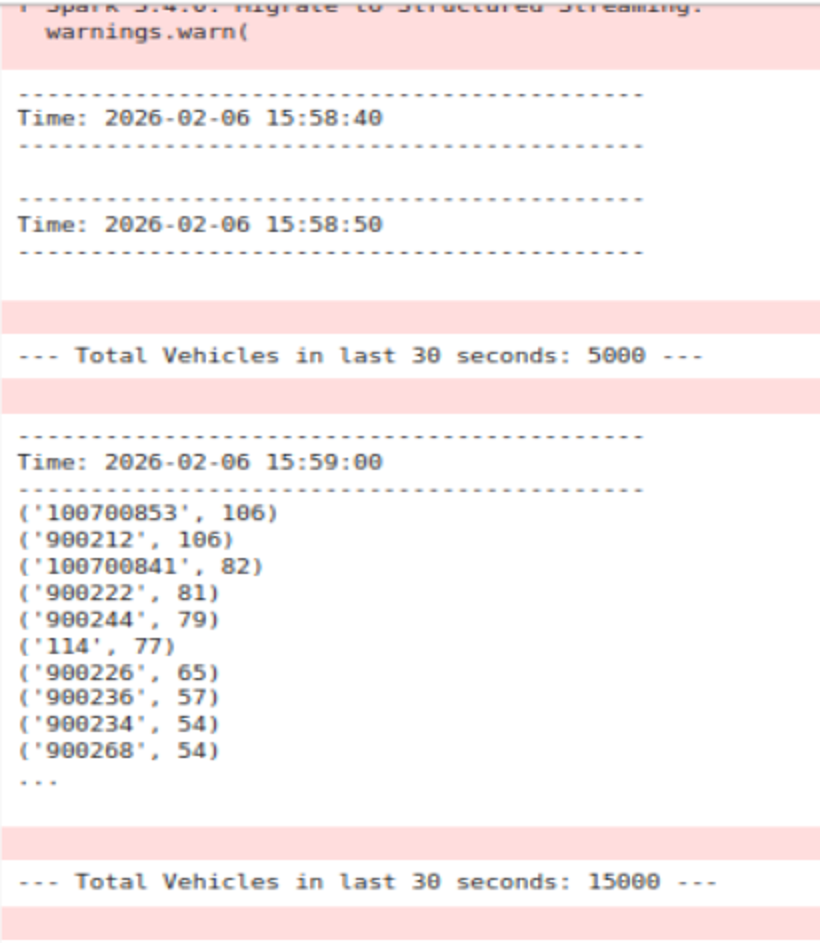
\includegraphics[width=\linewidth,height=.72\textheight,keepaspectratio]{assets/036_p018_01_panel1.png}\caption{Diagram or recorded result: Volume windows and top-three cameras. Panel 1 of 2.}\label{fig:036_p018_010}\end{figure}

\begin{figure}[!htbp]\centering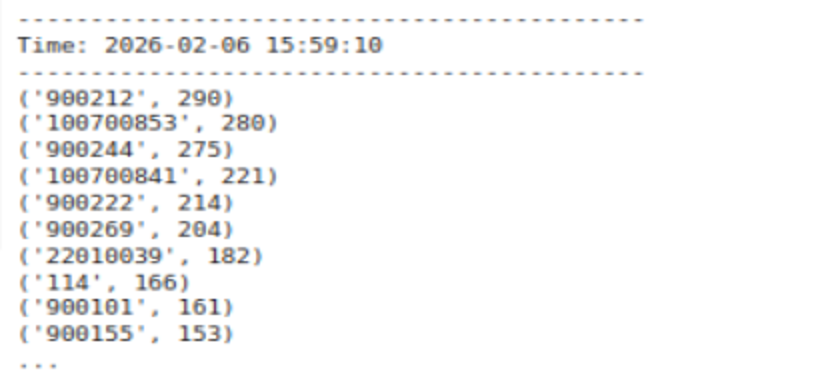
\includegraphics[width=\linewidth,height=.72\textheight,keepaspectratio]{assets/036_p018_01_panel2.png}\caption{Diagram or recorded result: Volume windows and top-three cameras. Panel 2 of 2.}\label{fig:036_p018_011}\end{figure}
\begin{figure}[!htbp]\centering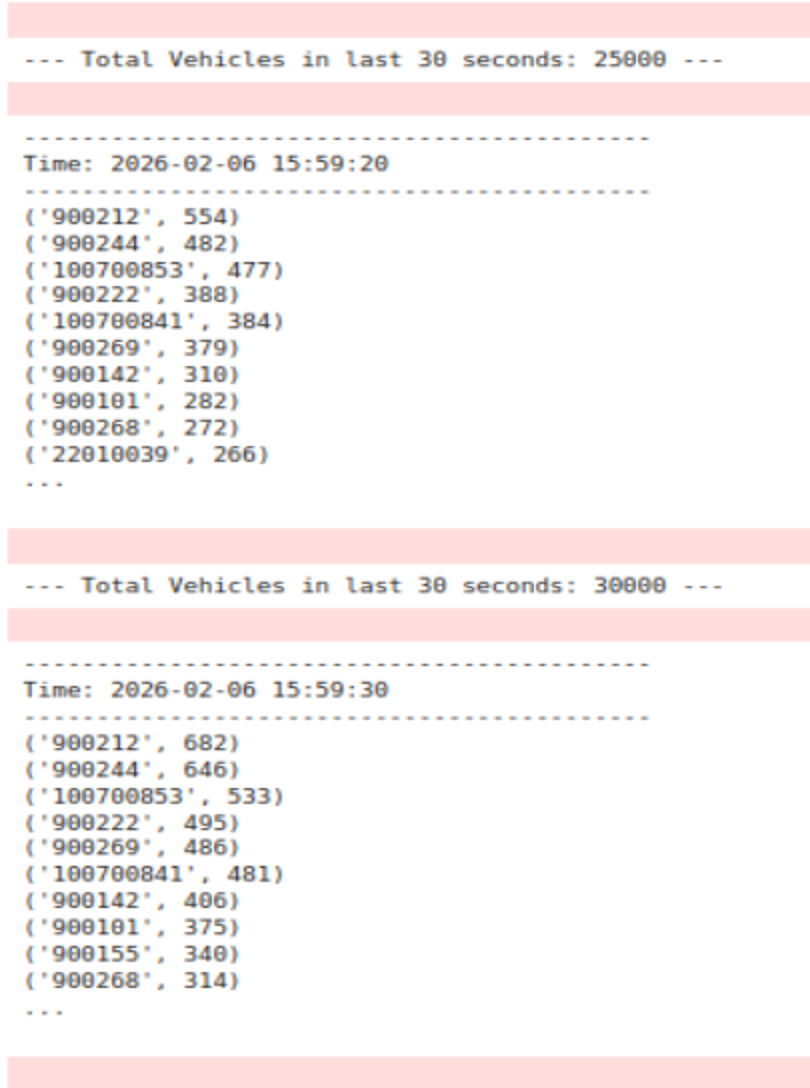
\includegraphics[width=\linewidth,height=.72\textheight,keepaspectratio]{assets/036_p018_02.png}\caption{Diagram or recorded result: Volume windows and top-three cameras.}\label{fig:036_p018_020}\end{figure}
\begin{figure}[!htbp]\centering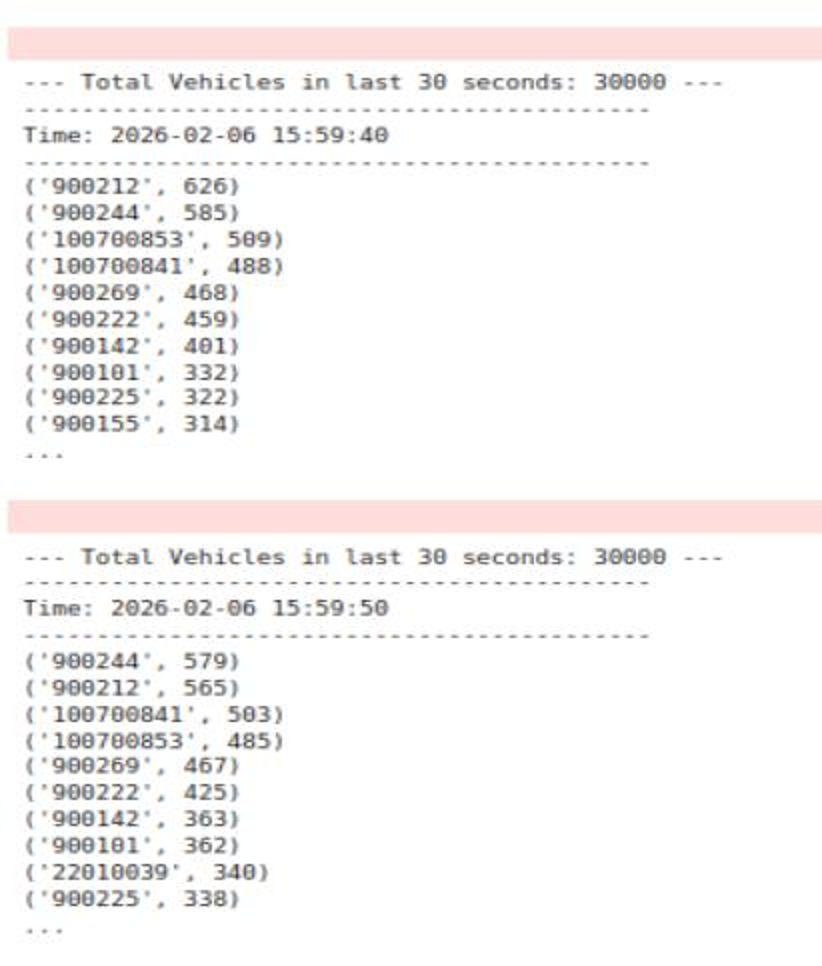
\includegraphics[width=\linewidth,height=.72\textheight,keepaspectratio]{assets/036_p018_03.png}\caption{Diagram or recorded result: Volume windows and top-three cameras.}\label{fig:036_p018_030}\end{figure}
\begin{figure}[!htbp]\centering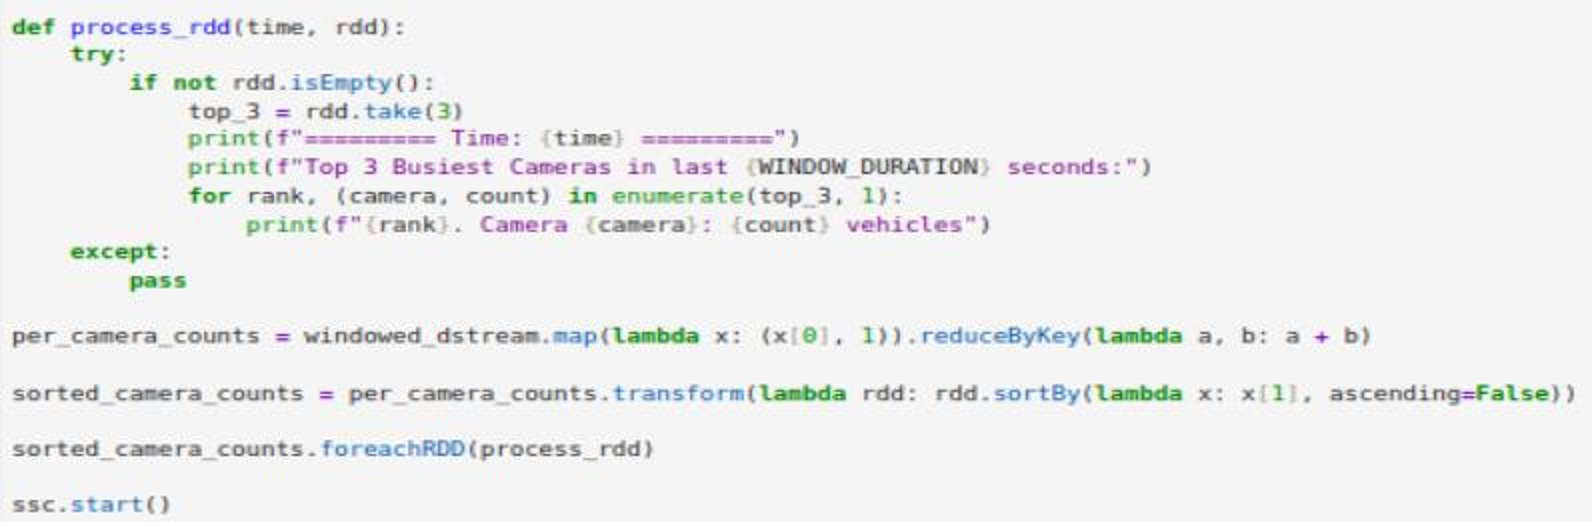
\includegraphics[width=\linewidth,height=.72\textheight,keepaspectratio]{assets/036_p019_02.png}\caption{Implementation and output: Volume windows and top-three cameras.}\label{fig:036_p019_020}\end{figure}
\begin{figure}[!htbp]\centering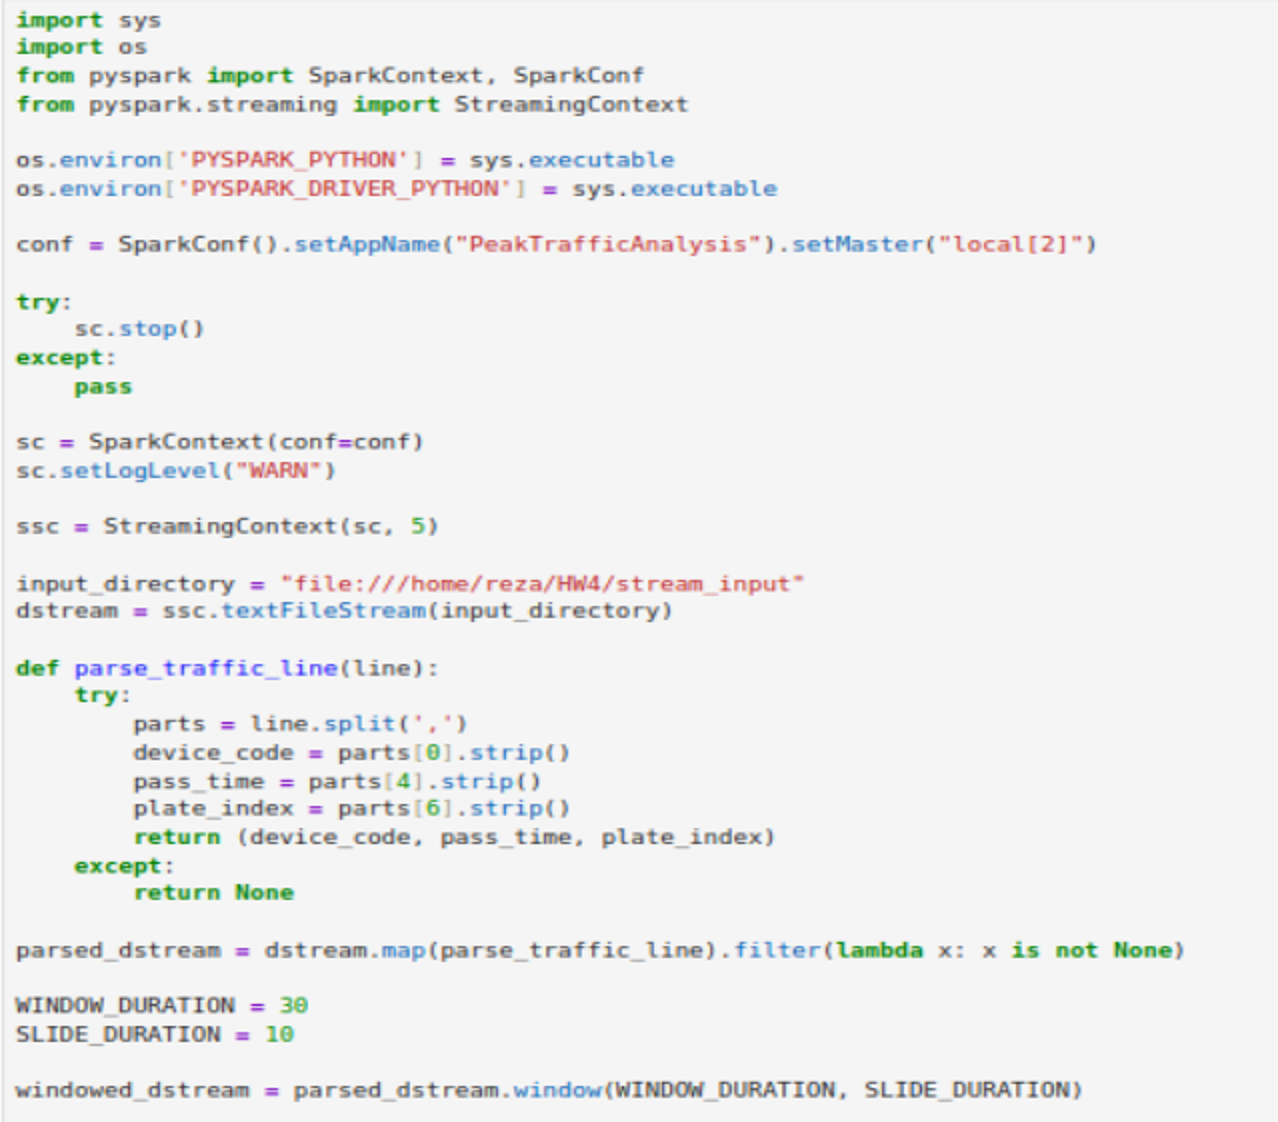
\includegraphics[width=\linewidth,height=.72\textheight,keepaspectratio]{assets/036_p019_03.png}\caption{Implementation and output: Volume windows and top-three cameras.}\label{fig:036_p019_030}\end{figure}
\clearpage
\section{Repeated plates and behavioral interpretation}

The behavioral query uses a sixty-second window, a ten-second slide, and threshold N=\allowbreak{}3:\allowbreak{} plates with at least four recorded observations qualify. N is a parameter. Longer windows capture more repeated observations but require more distinct-key state and can combine unrelated events. Shorter windows can separate occurrences that a longer interval would group. Repeated plate observations do not prove multiple distinct camera visits, speeding, prohibited travel, or suspicious intent. Those interpretations require validated identities, locations, travel times, and camera deduplication. The recorded physical-distance explanation is especially inappropriate when timestamps are replayed at a different wall-clock rate.

\begin{figure}[!htbp]\centering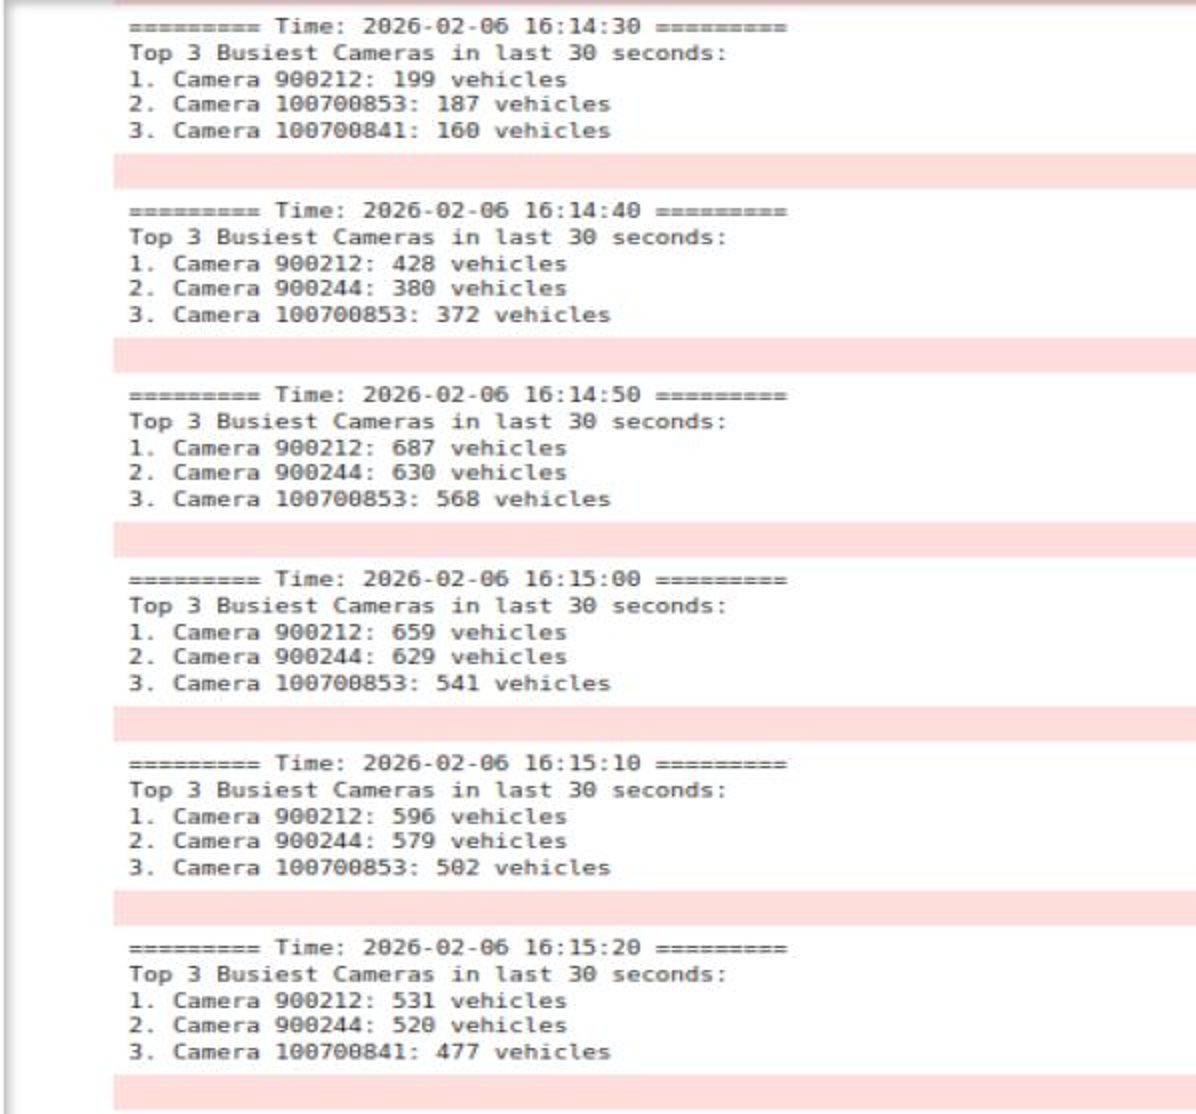
\includegraphics[width=\linewidth,height=.72\textheight,keepaspectratio]{assets/036_p020_01.png}\caption{Diagram or recorded result: Repeated plates and behavioral interpretation.}\label{fig:036_p020_010}\end{figure}
\begin{figure}[!htbp]\centering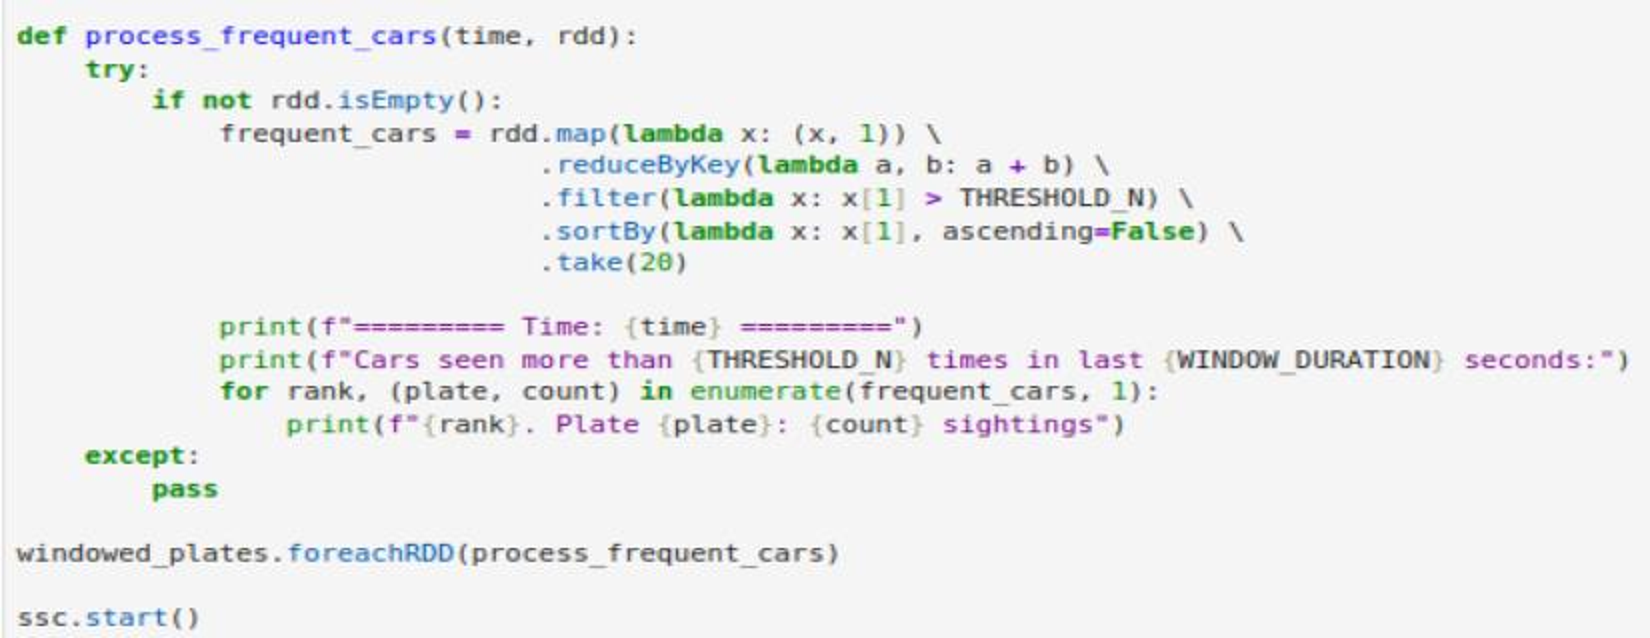
\includegraphics[width=\linewidth,height=.72\textheight,keepaspectratio]{assets/036_p022_01.png}\caption{Implementation and output: Repeated plates and behavioral interpretation.}\label{fig:036_p022_010}\end{figure}
\begin{figure}[!htbp]\centering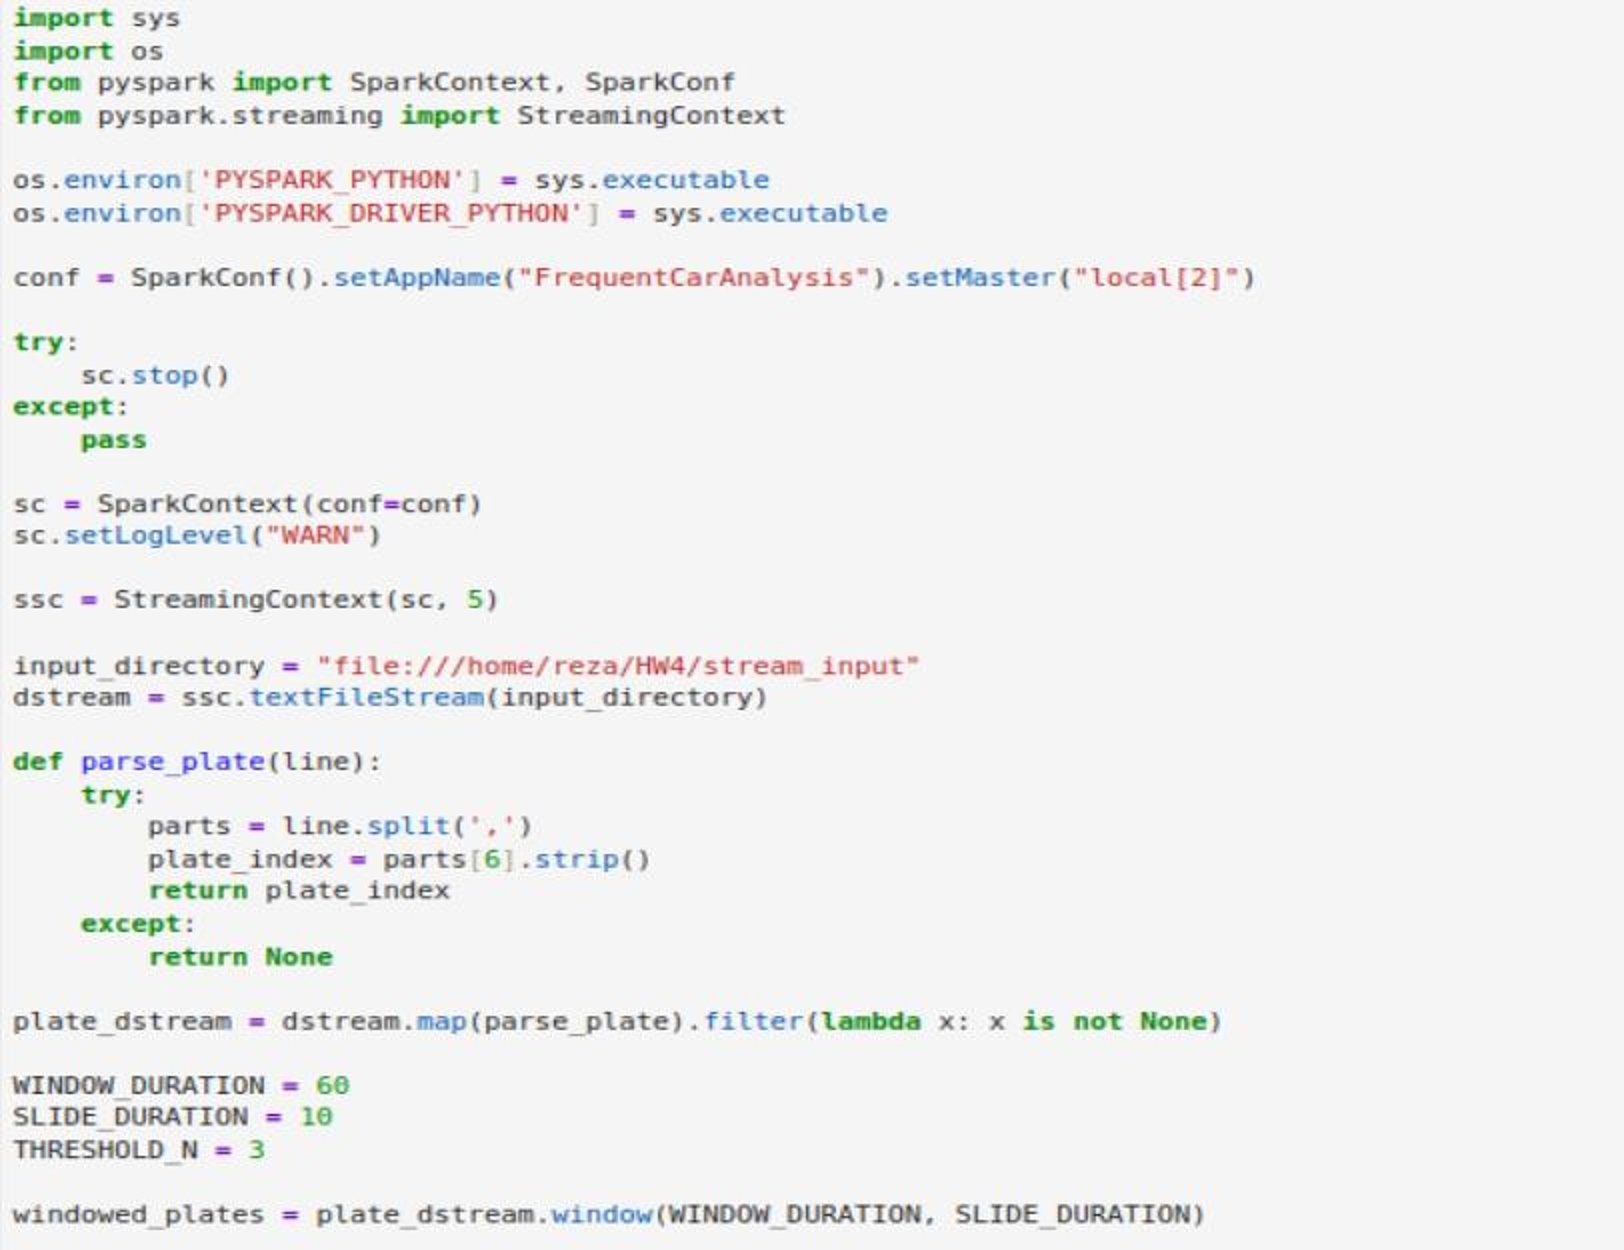
\includegraphics[width=\linewidth,height=.72\textheight,keepaspectratio]{assets/036_p022_02.png}\caption{Implementation and output: Repeated plates and behavioral interpretation.}\label{fig:036_p022_020}\end{figure}
\begin{figure}[!htbp]\centering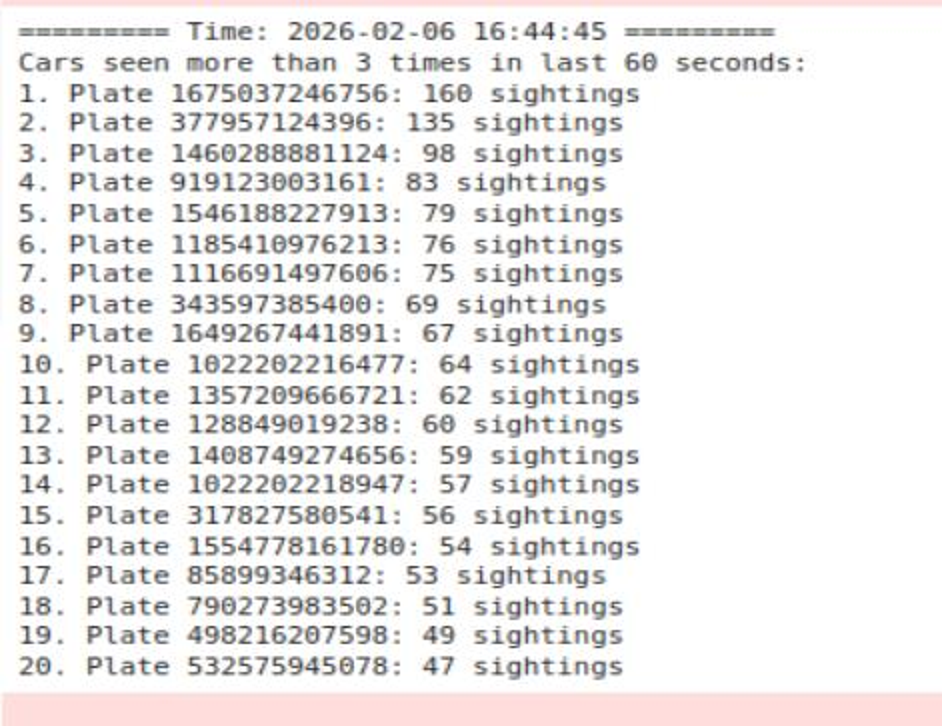
\includegraphics[width=\linewidth,height=.72\textheight,keepaspectratio]{assets/036_p023_01.png}\caption{Diagram or recorded result: Repeated plates and behavioral interpretation.}\label{fig:036_p023_010}\end{figure}
\begin{figure}[!htbp]\centering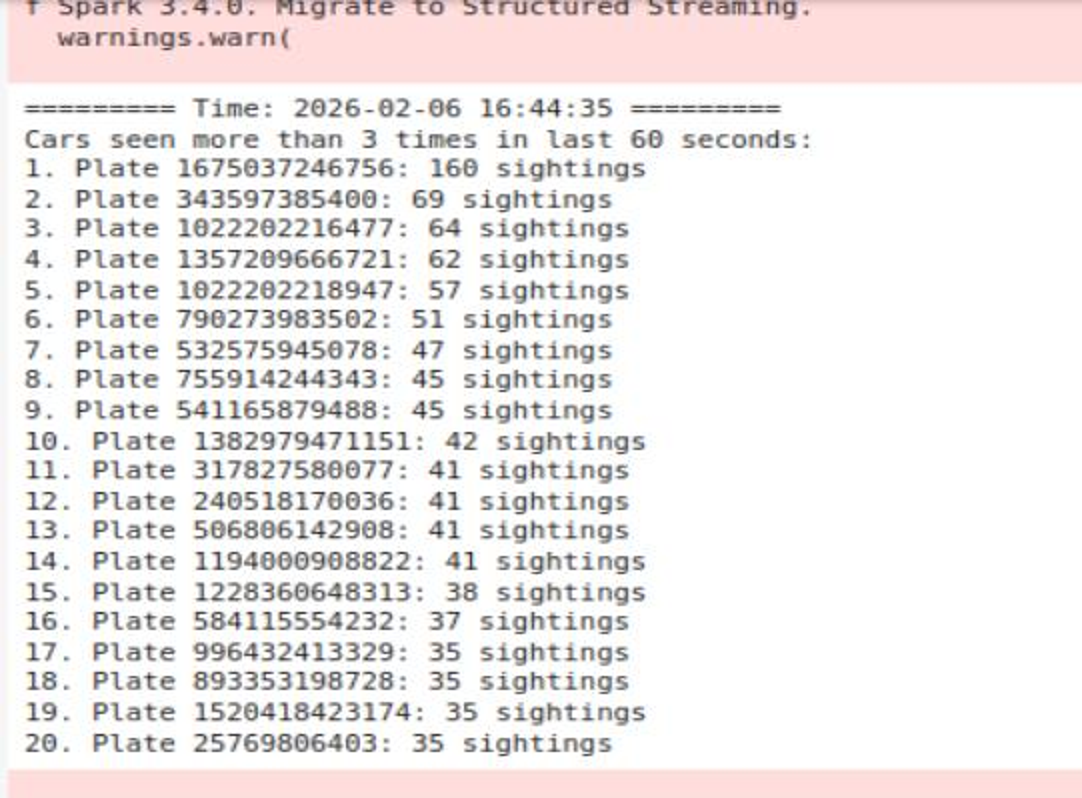
\includegraphics[width=\linewidth,height=.72\textheight,keepaspectratio]{assets/036_p023_02.png}\caption{Diagram or recorded result: Repeated plates and behavioral interpretation.}\label{fig:036_p023_020}\end{figure}
\begin{figure}[!htbp]\centering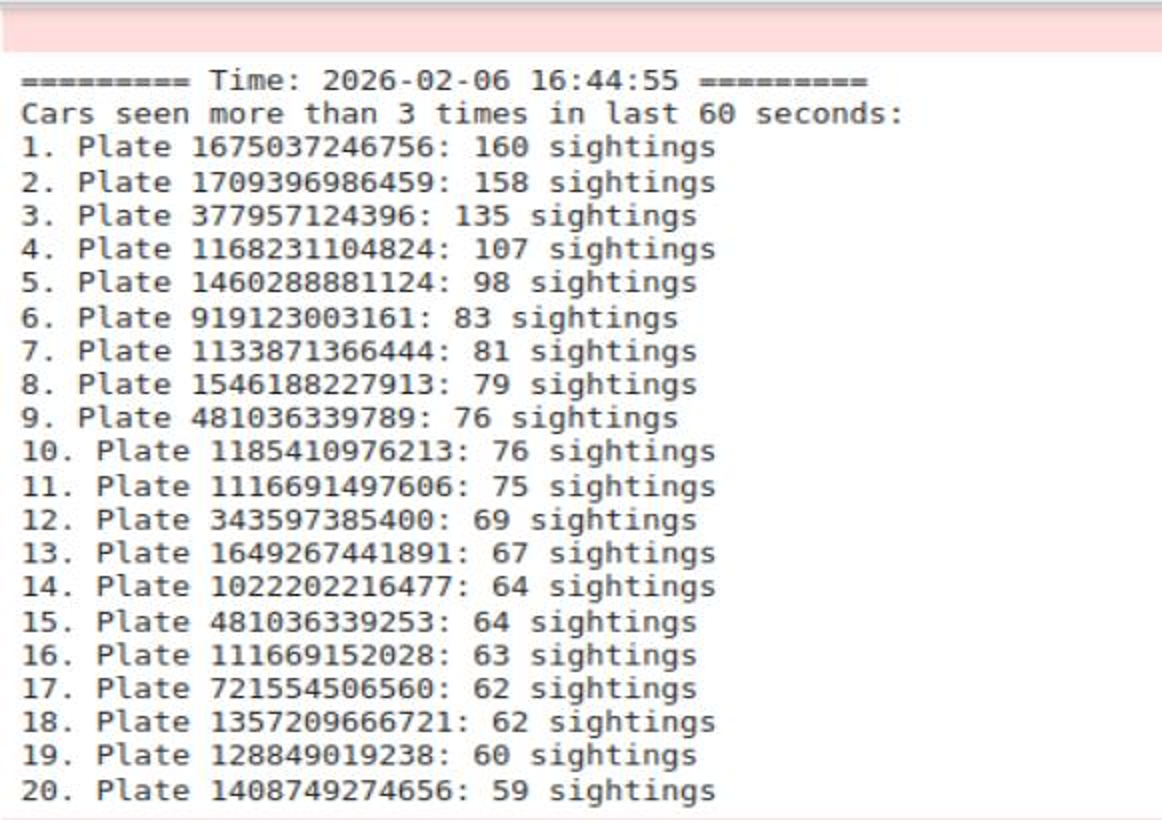
\includegraphics[width=\linewidth,height=.72\textheight,keepaspectratio]{assets/036_p023_03.png}\caption{Diagram or recorded result: Repeated plates and behavioral interpretation.}\label{fig:036_p023_030}\end{figure}
\begin{figure}[!htbp]\centering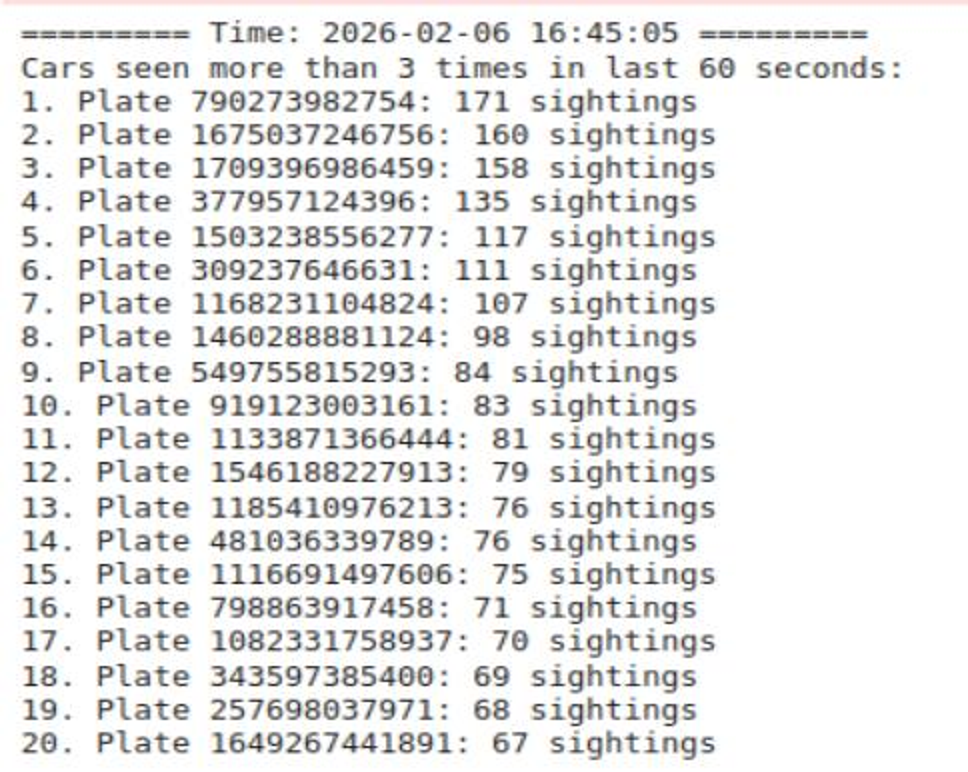
\includegraphics[width=\linewidth,height=.72\textheight,keepaspectratio]{assets/036_p023_04.png}\caption{Diagram or recorded result: Repeated plates and behavioral interpretation.}\label{fig:036_p023_040}\end{figure}
\clearpage
\section{Camera diversity}

A sixty-second window with a twenty-second slide computes total observations per camera and distinct (camera,plate) pairs. Joining these counts gives diversity=\allowbreak{}UniquePlates/\allowbreak{}TotalPasses, between zero and one for nonempty windows. A low ratio indicates repeat observations, which may reflect congestion, duplicate detections, loops, parking movements, or sensor behavior. It does not uniquely identify a road type. The report filters TotalPasses>100 and diversity<0.6. Its example camera 100701262 has 155 observations and 33 distinct plates:\allowbreak{} 33/\allowbreak{}155=\allowbreak{}0.2129032, or about 4.697 observations per distinct plate. A low-diversity camera is not proven to be outside a highway. Changing window length changes which repeats are grouped;\allowbreak{} more data can help interpretation while also reducing temporal specificity.

\begin{figure}[!htbp]\centering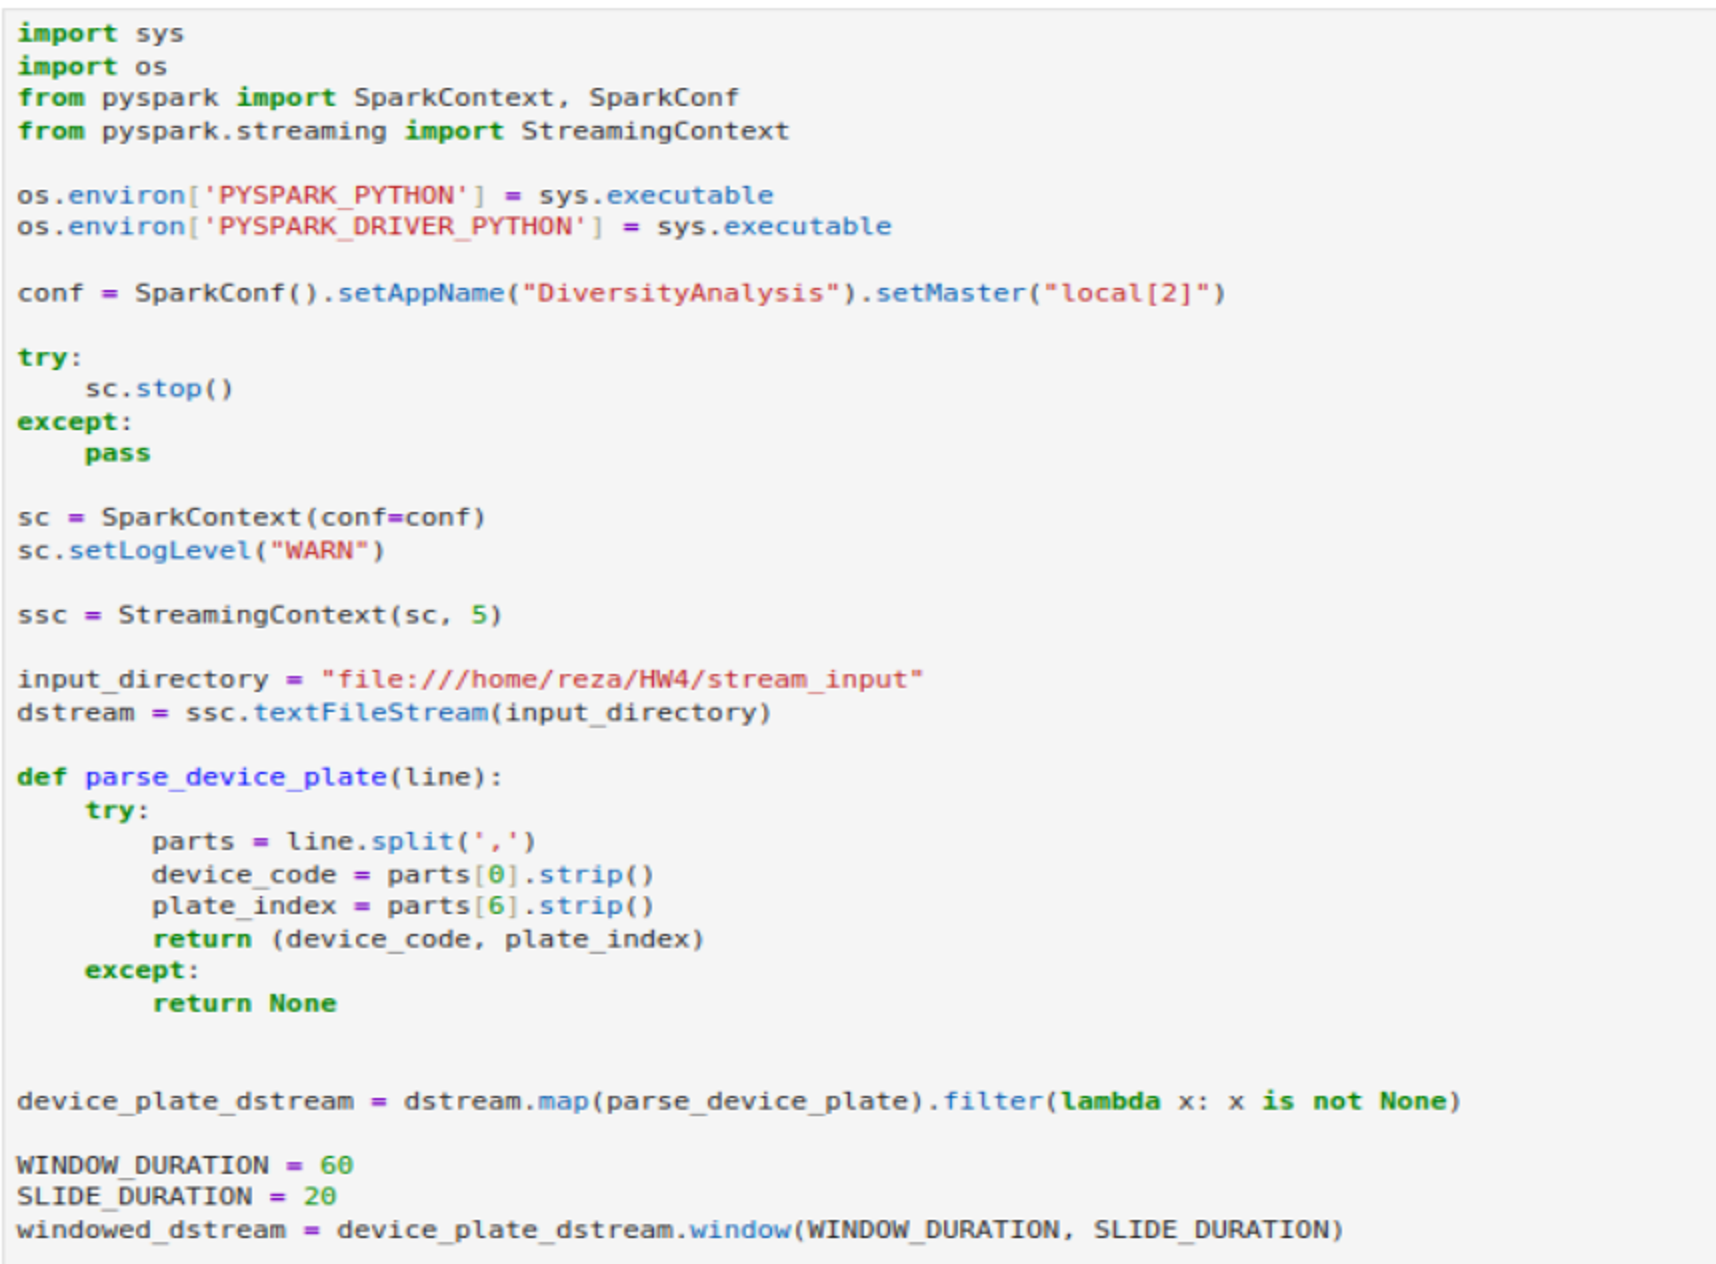
\includegraphics[width=\linewidth,height=.72\textheight,keepaspectratio]{assets/036_p025_02.png}\caption{Implementation and output: Camera diversity.}\label{fig:036_p025_020}\end{figure}
\begin{figure}[!htbp]\centering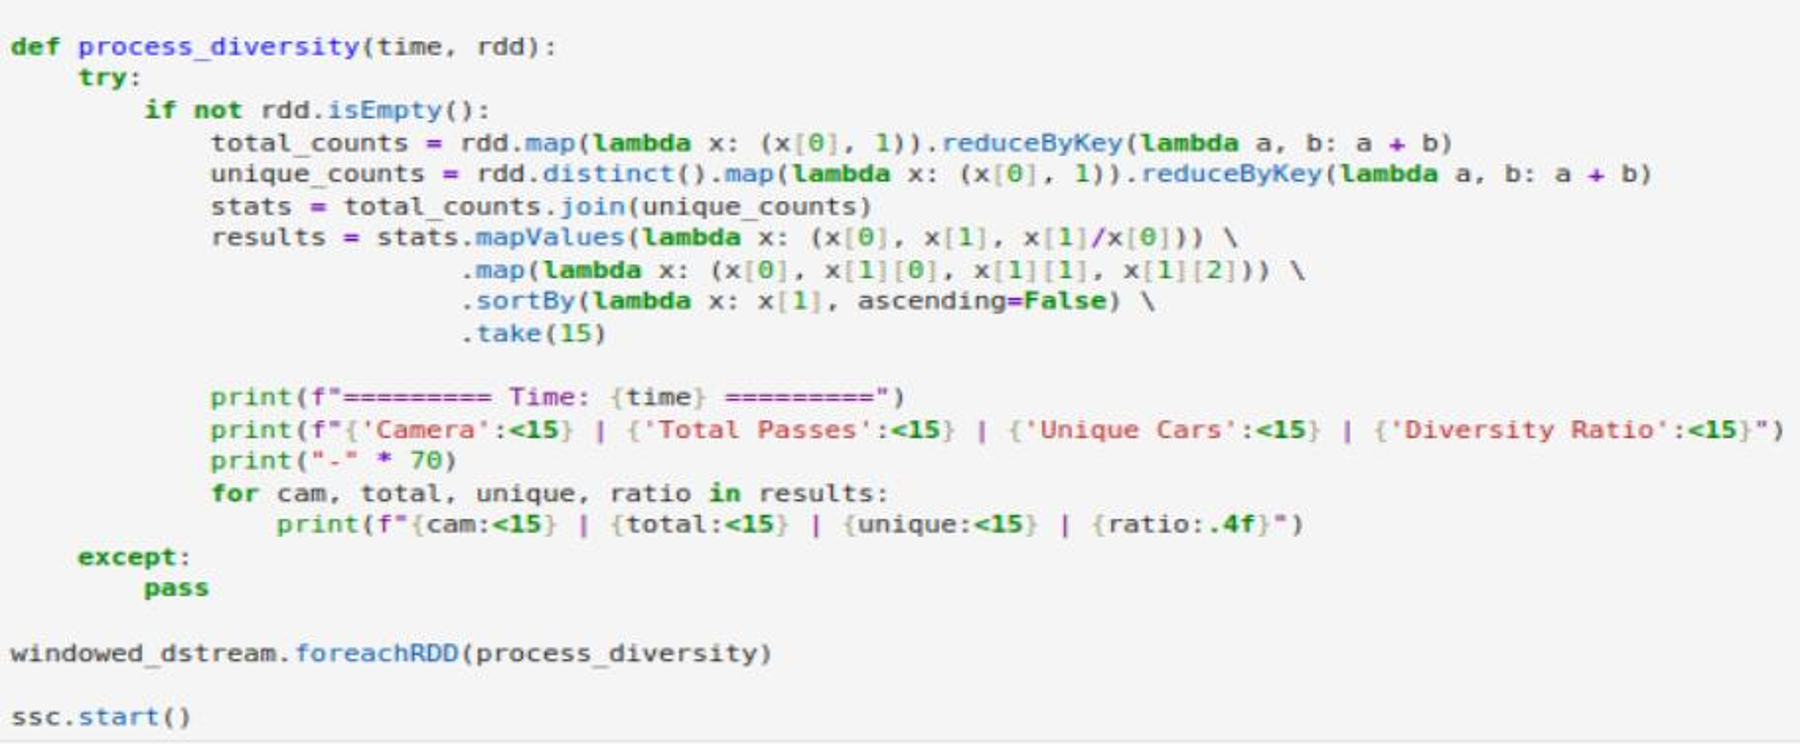
\includegraphics[width=\linewidth,height=.72\textheight,keepaspectratio]{assets/036_p025_03.png}\caption{Implementation and output: Camera diversity.}\label{fig:036_p025_030}\end{figure}
\begin{figure}[!htbp]\centering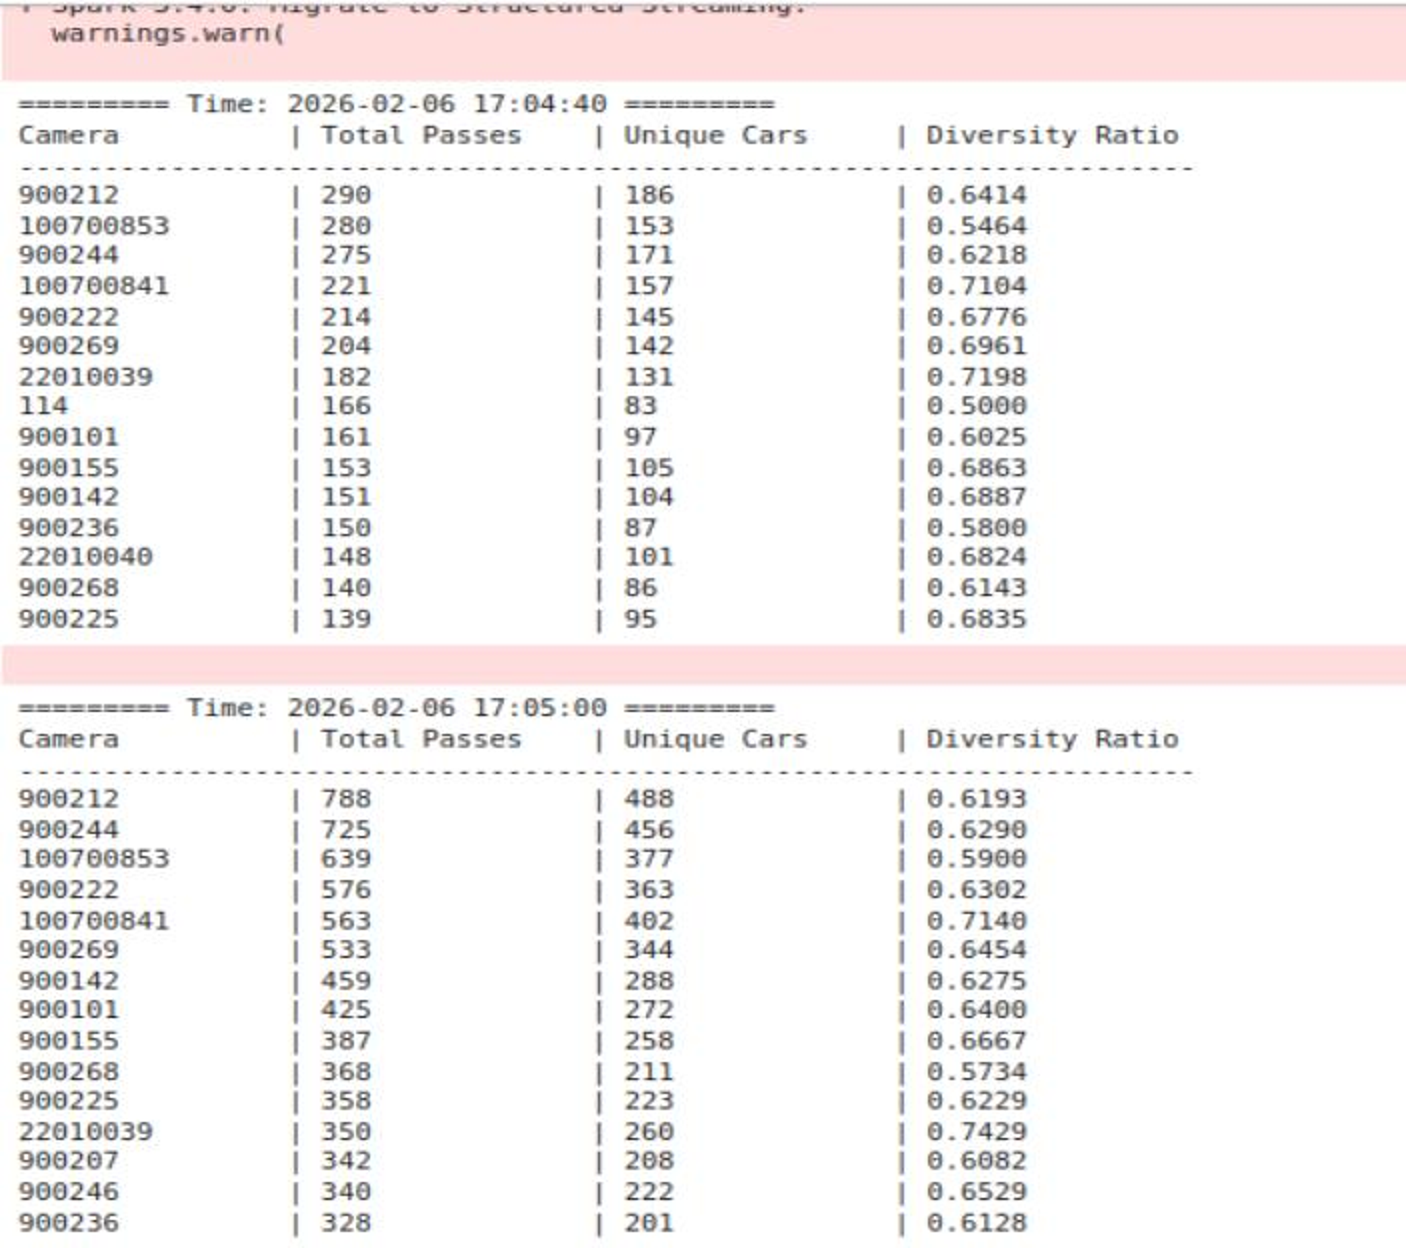
\includegraphics[width=\linewidth,height=.72\textheight,keepaspectratio]{assets/036_p026_01.png}\caption{Diagram or recorded result: Camera diversity.}\label{fig:036_p026_010}\end{figure}
\begin{figure}[!htbp]\centering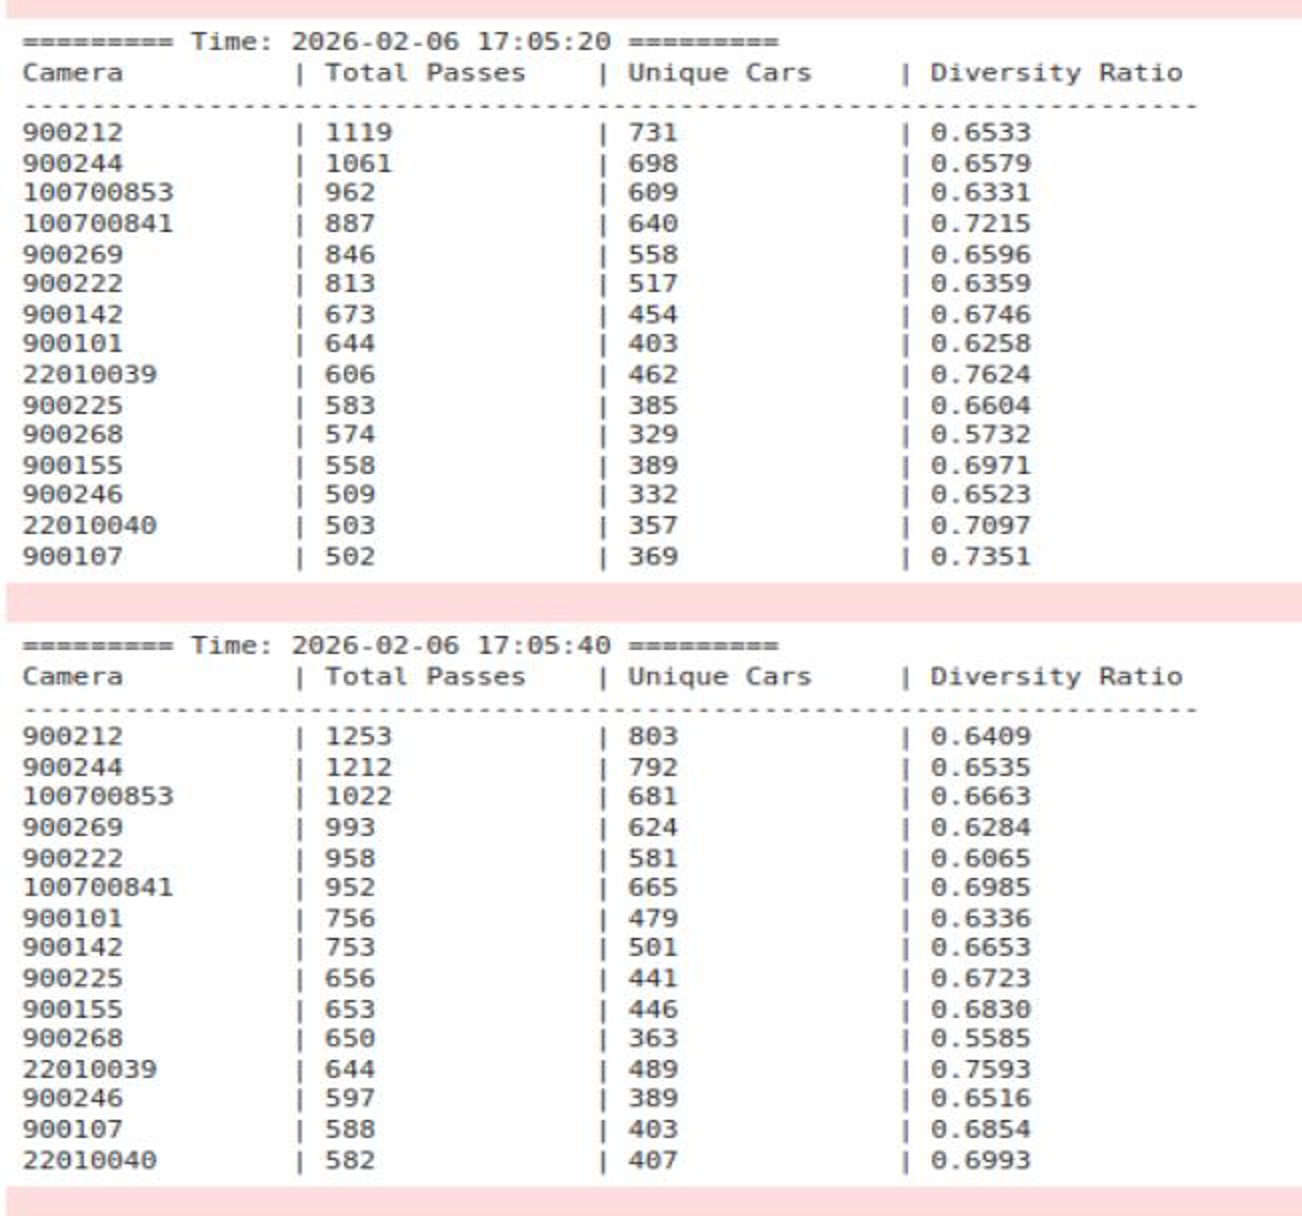
\includegraphics[width=\linewidth,height=.72\textheight,keepaspectratio]{assets/036_p026_02.png}\caption{Diagram or recorded result: Camera diversity.}\label{fig:036_p026_020}\end{figure}
\begin{figure}[!htbp]\centering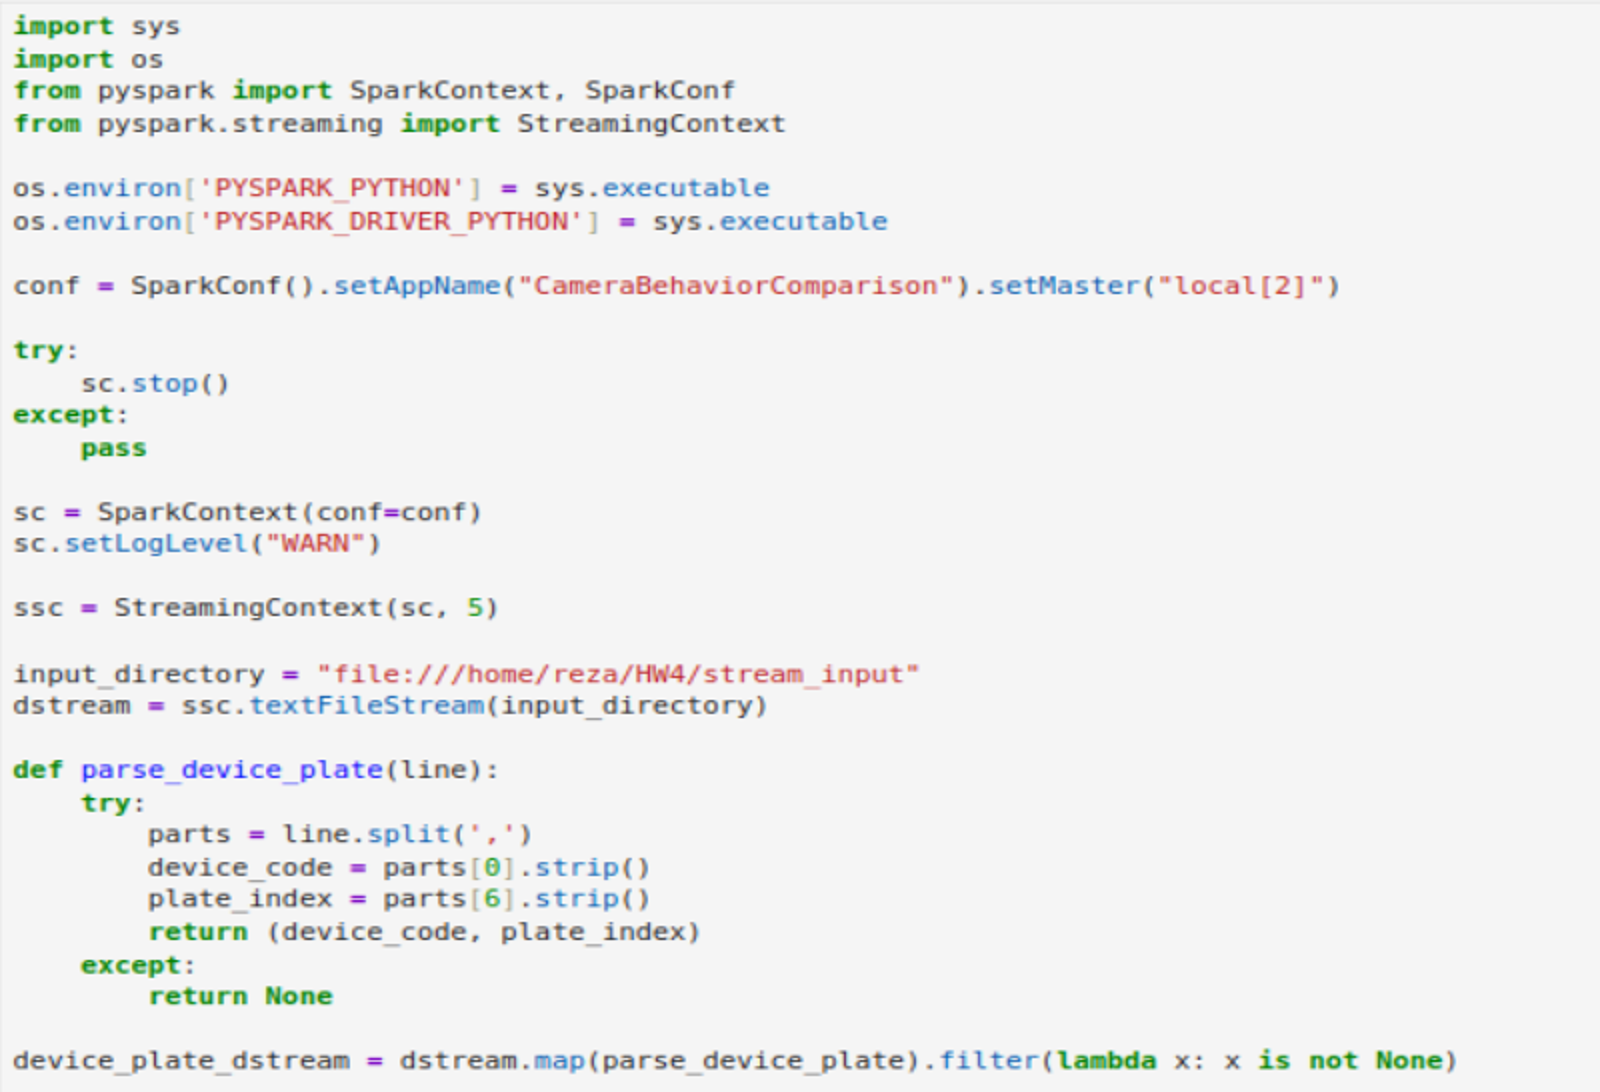
\includegraphics[width=\linewidth,height=.72\textheight,keepaspectratio]{assets/036_p029_02.png}\caption{Implementation and output: Camera diversity.}\label{fig:036_p029_020}\end{figure}
\begin{figure}[!htbp]\centering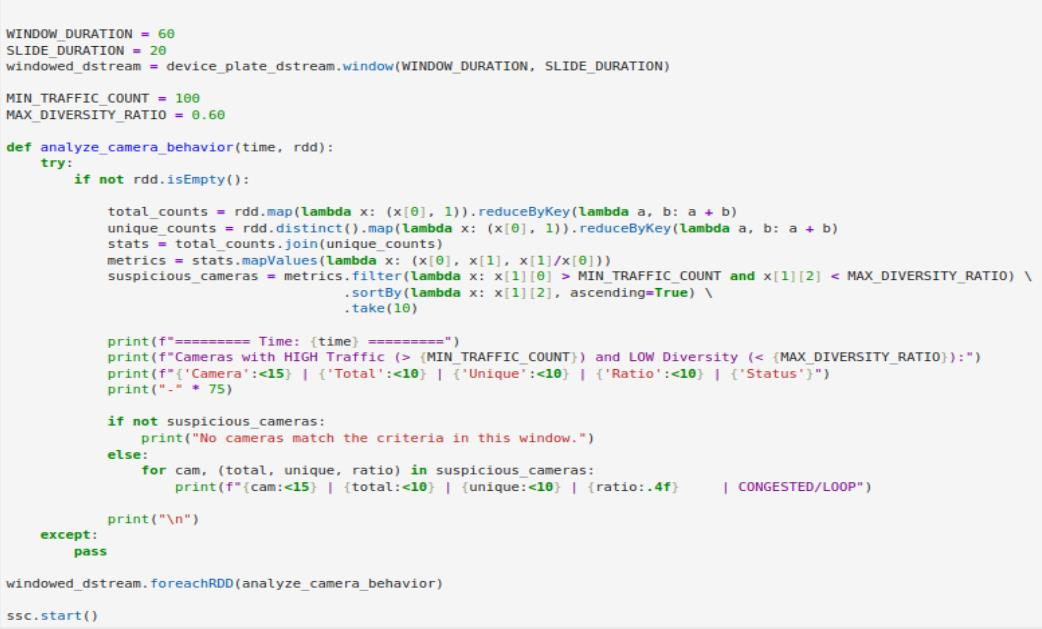
\includegraphics[width=\linewidth,height=.72\textheight,keepaspectratio]{assets/036_p029_03.png}\caption{Implementation and output: Camera diversity.}\label{fig:036_p029_030}\end{figure}
\begin{figure}[!htbp]\centering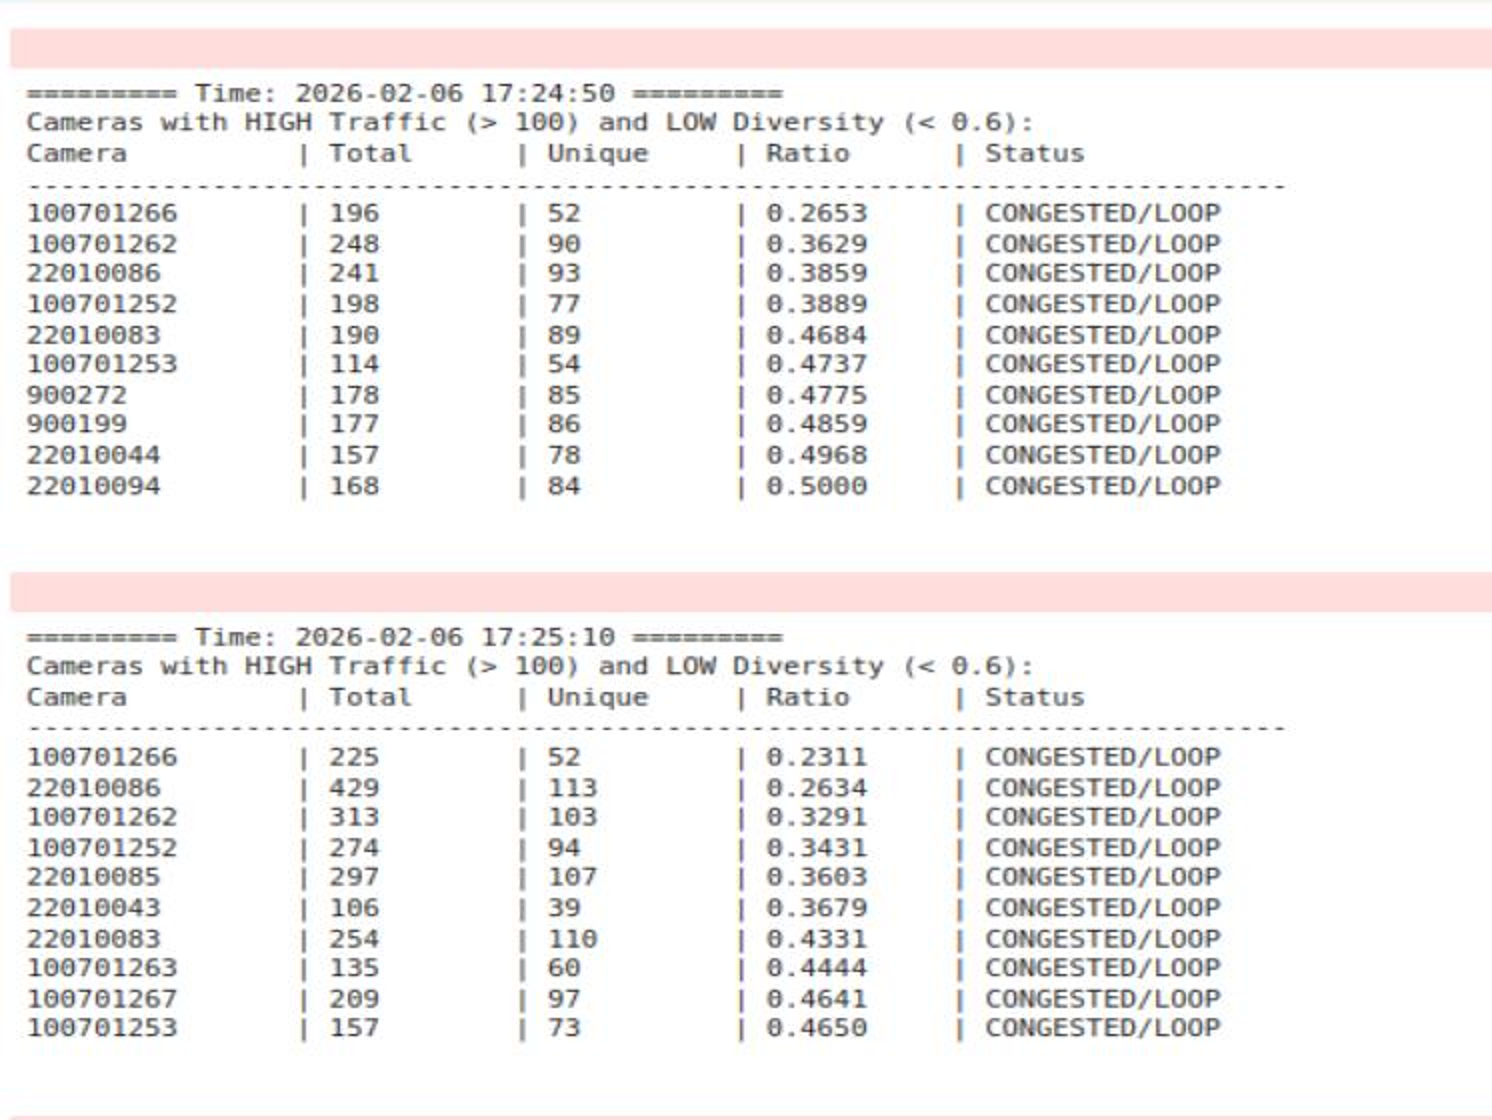
\includegraphics[width=\linewidth,height=.72\textheight,keepaspectratio]{assets/036_p030_01.png}\caption{Diagram or recorded result: Camera diversity.}\label{fig:036_p030_010}\end{figure}
\begin{figure}[!htbp]\centering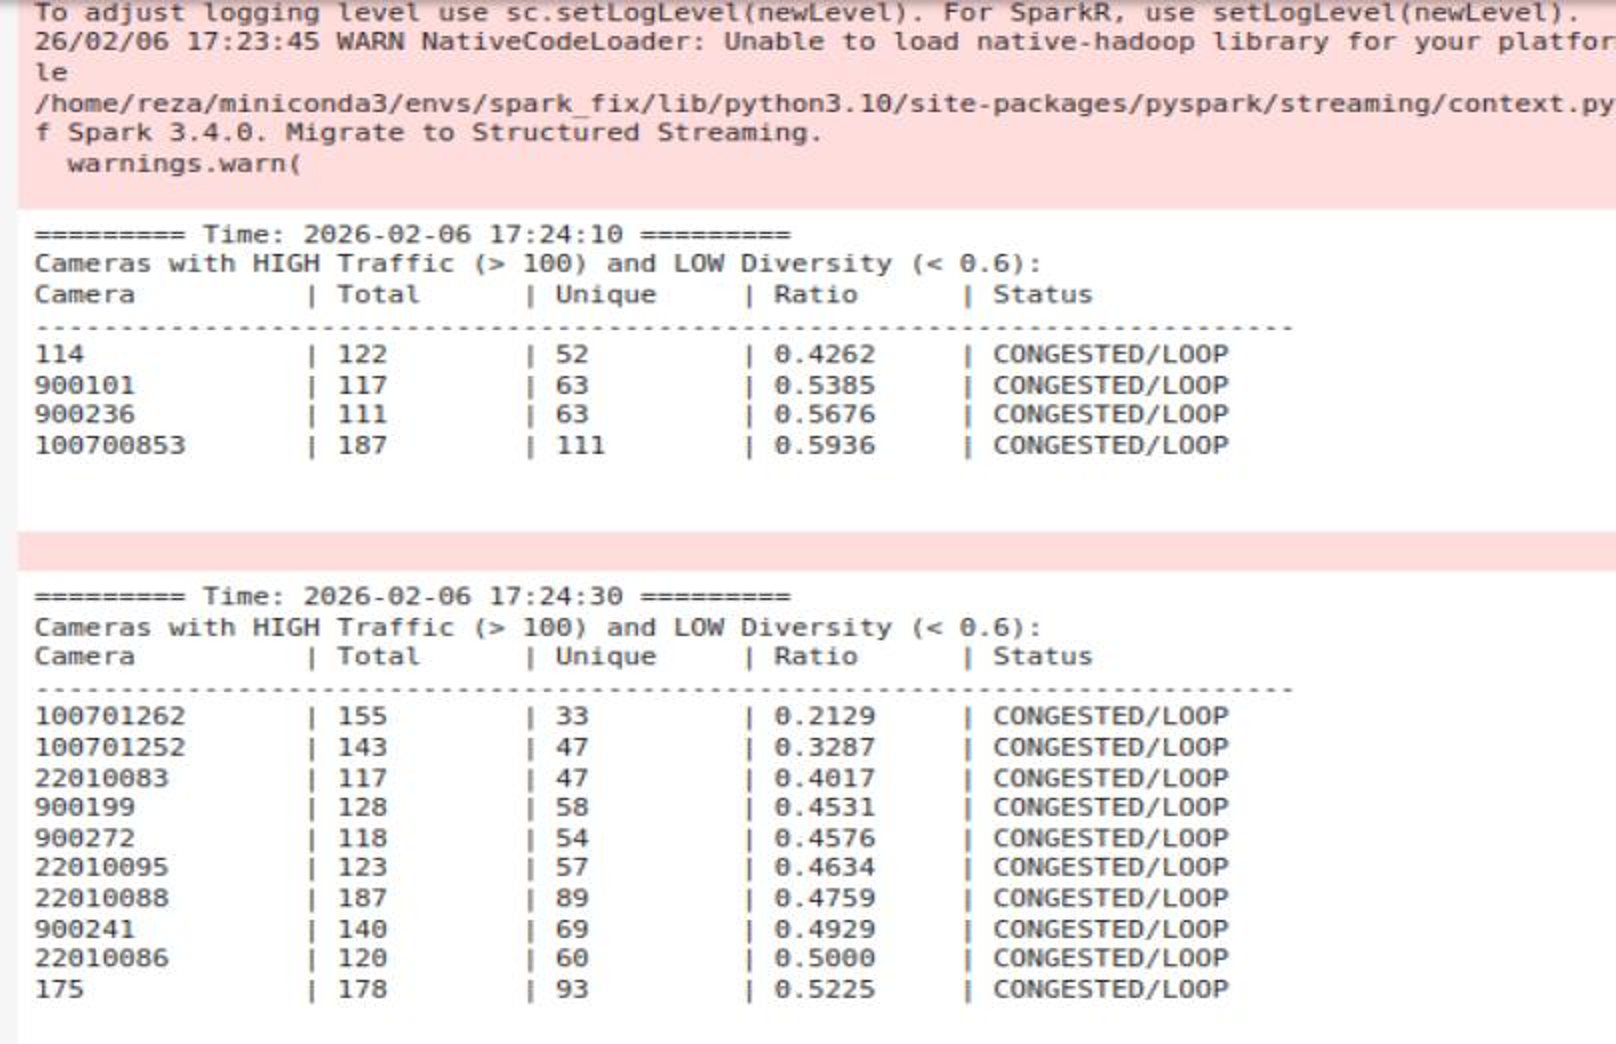
\includegraphics[width=\linewidth,height=.72\textheight,keepaspectratio]{assets/036_p030_02.png}\caption{Implementation and output: Camera diversity.}\label{fig:036_p030_020}\end{figure}
\begin{figure}[!htbp]\centering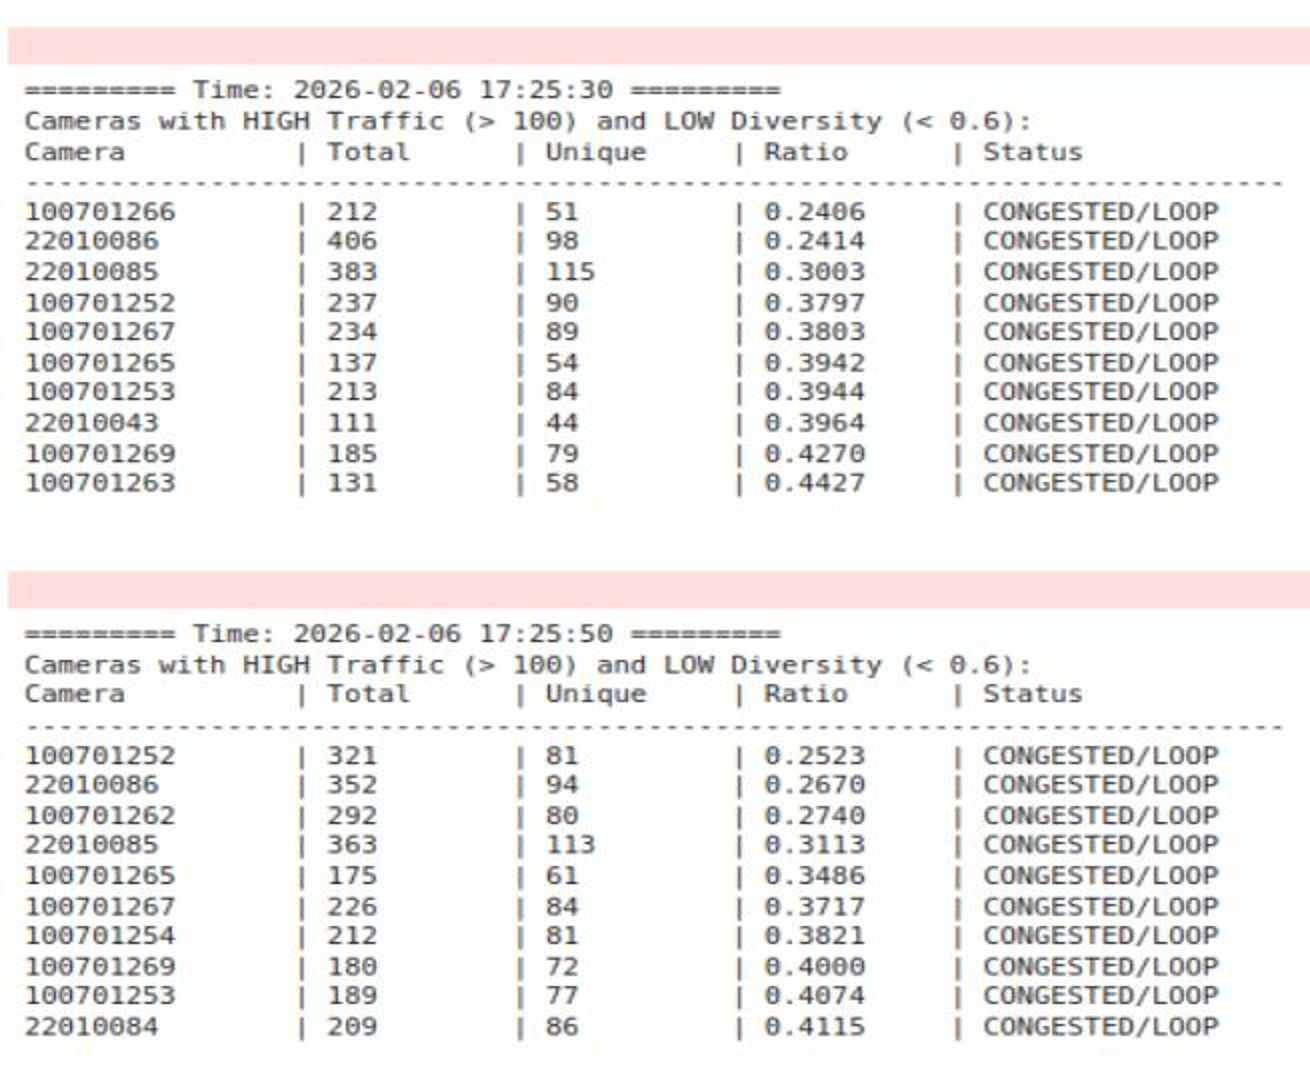
\includegraphics[width=\linewidth,height=.72\textheight,keepaspectratio]{assets/036_p030_03.png}\caption{Diagram or recorded result: Camera diversity.}\label{fig:036_p030_030}\end{figure}
\clearpage
\section{Practical 2: four-hash distinct counting}

camera\_\allowbreak{}passes.csv supplies CameraID and PlateNumber. Each plate is hashed with md5, sha1, sha224, and sha256;\allowbreak{} the maximum trailing-zero register for each hash is maintained. The report combines the four registers by their median and uses 2 raised to that median as its estimate. This reduces the influence of one exceptionally large register, but four hashes still have high variance. If the median of an even number of registers is their middle-pair average, its value can be half-integer and the estimate need not be an integer power of two.


\begingroup\small\setlength{\tabcolsep}{3pt}\renewcommand{\arraystretch}{1.2}
\begin{longtable}{@{}p{0.2263\linewidth}p{0.2263\linewidth}p{0.2263\linewidth}p{0.2263\linewidth}@{}}
\toprule
\textbf{Submitted sample} & \textbf{Exact distinct} & \textbf{Reported estimate} & \textbf{Absolute relative error} \\ \midrule
\endfirsthead
\textbf{Submitted sample} & \textbf{Exact distinct} & \textbf{Reported estimate} & \textbf{Absolute relative error} \\ \midrule \endhead
Global sample 1 & 1793 & 2896 & 61.5170\% \\
Global sample 2 & 3318 & 4870 & 46.7752\% \\
\bottomrule\end{longtable}\endgroup

The exact reference is distinct().count(). Four registers provide a small sketch, while the exact reference requires work/\allowbreak{}state proportional to observed distinct items. The errors illustrate the weakness of this simple estimator;\allowbreak{} they are not a demonstrated accuracy guarantee or an inevitable fixed error range. The pipeline's exact-evaluation operations also consume resources, so the complete experiment cannot be described as constant-memory merely because the register summary is small. For expiring windows, a cumulative maximum register cannot simply forget old items. Recomputing a sketch for each window or using an explicitly window-aware structure is necessary. This distinction should be checked against the notebook before interpreting a cumulative result as a sliding-window estimate.

\begin{figure}[!htbp]\centering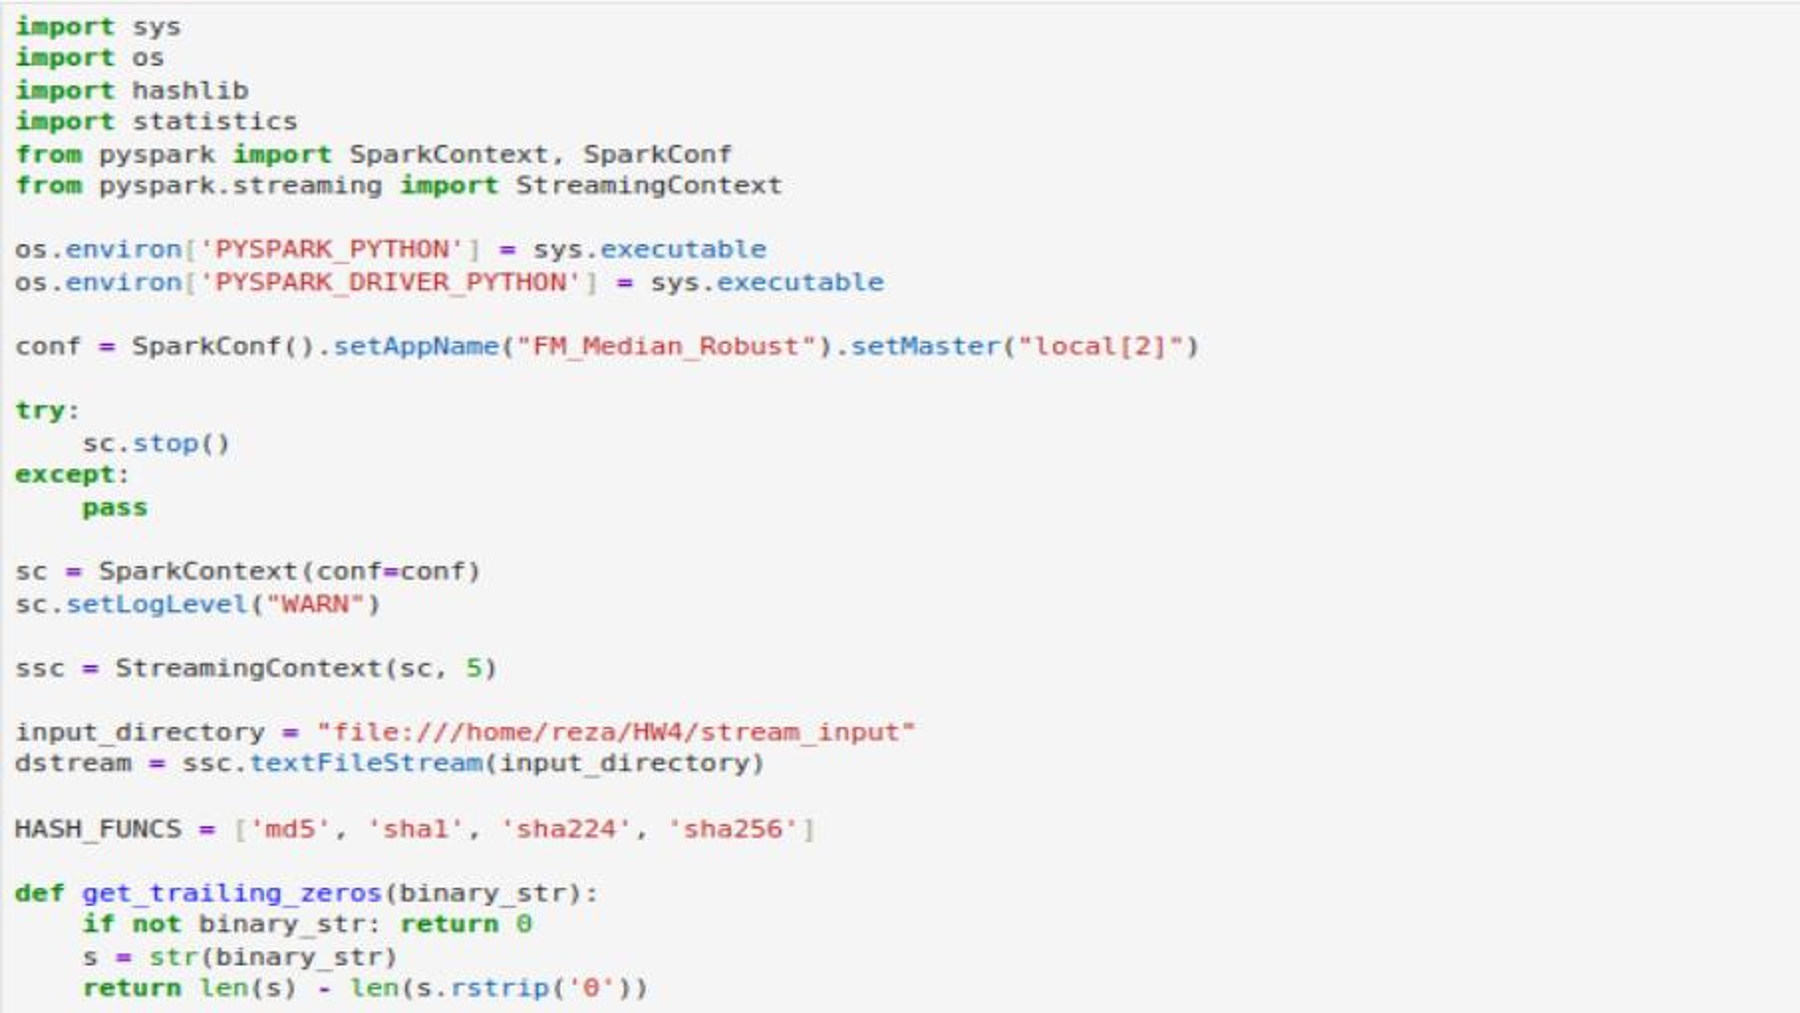
\includegraphics[width=\linewidth,height=.72\textheight,keepaspectratio]{assets/036_p033_01.png}\caption{Implementation and output: Practical 2: four-hash distinct counting.}\label{fig:036_p033_010}\end{figure}
\begin{figure}[!htbp]\centering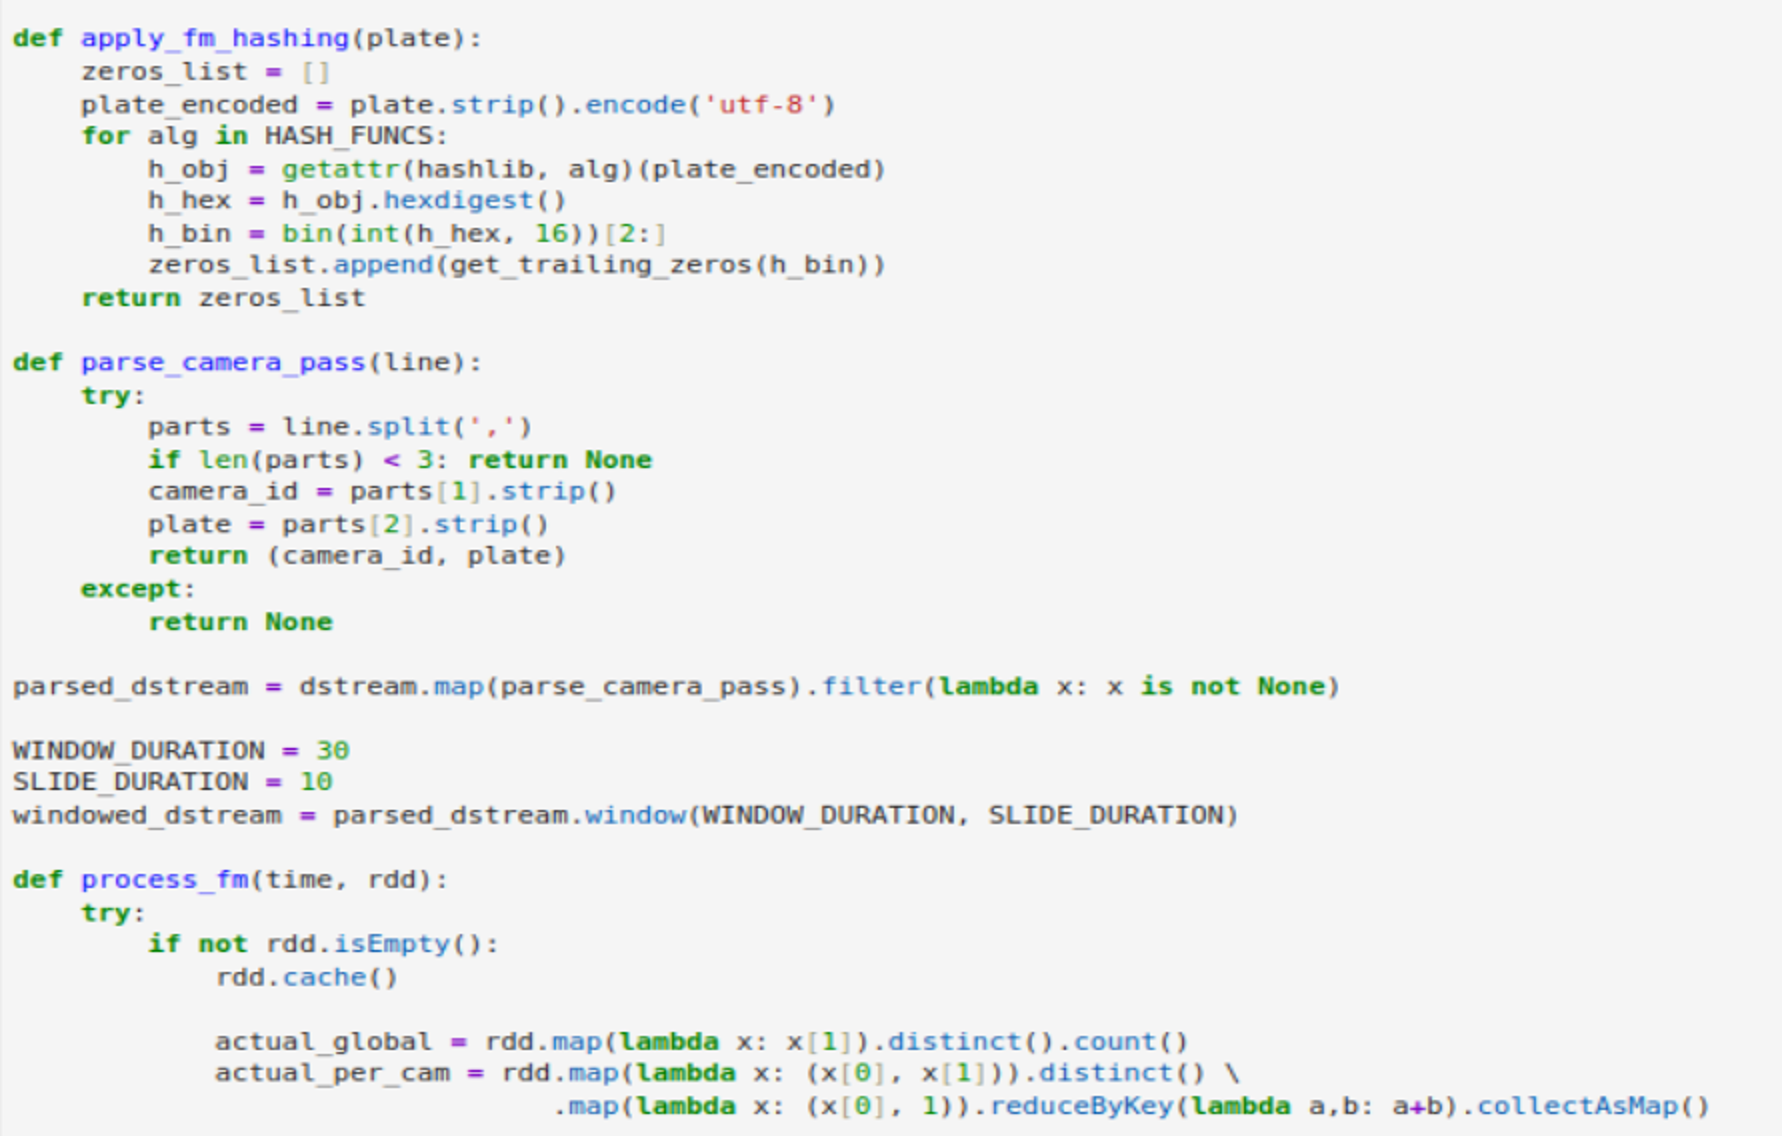
\includegraphics[width=\linewidth,height=.72\textheight,keepaspectratio]{assets/036_p033_02.png}\caption{Implementation and output: Practical 2: four-hash distinct counting.}\label{fig:036_p033_020}\end{figure}
\begin{figure}[!htbp]\centering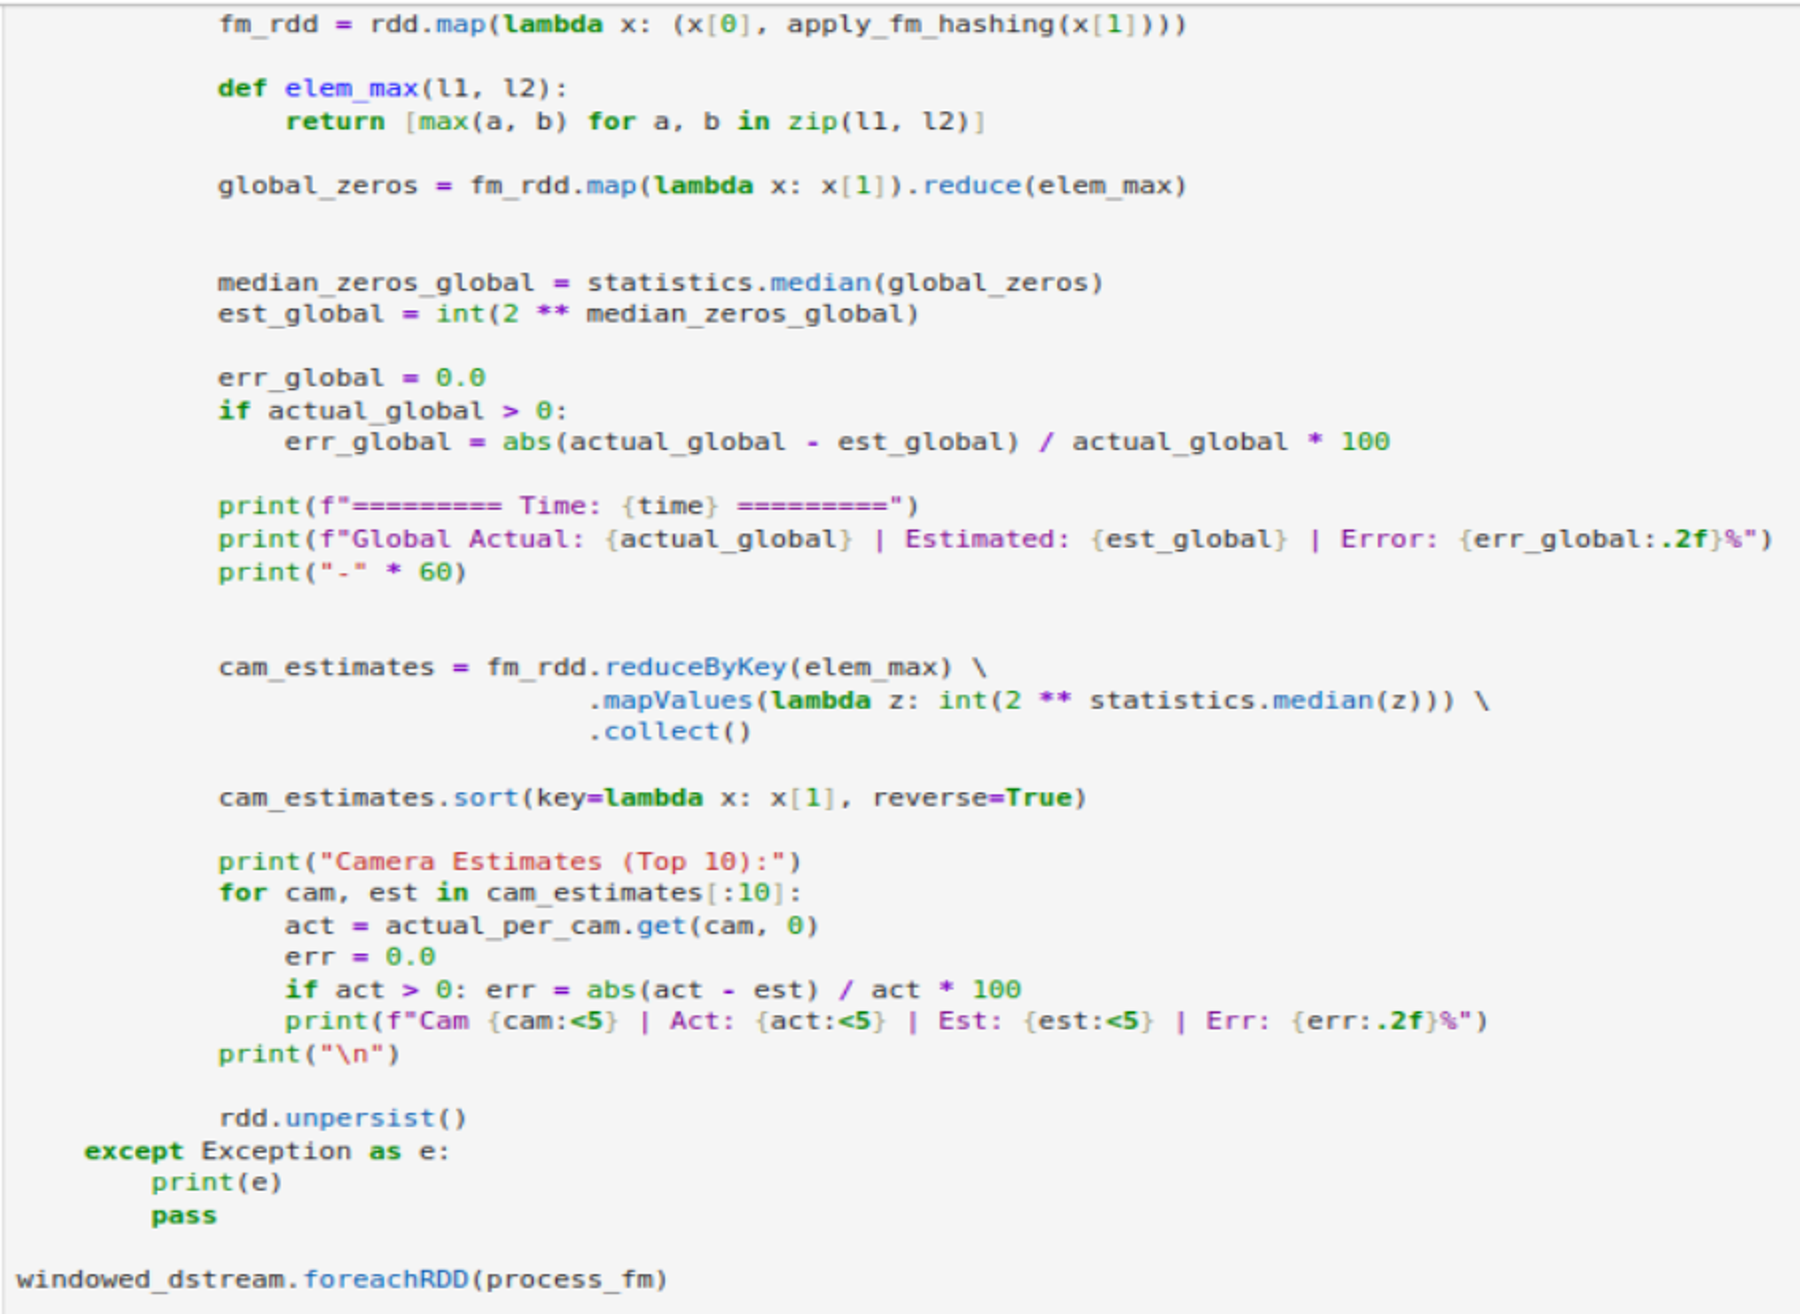
\includegraphics[width=\linewidth,height=.72\textheight,keepaspectratio]{assets/036_p033_03.png}\caption{Implementation and output: Practical 2: four-hash distinct counting.}\label{fig:036_p033_030}\end{figure}
\begin{figure}[!htbp]\centering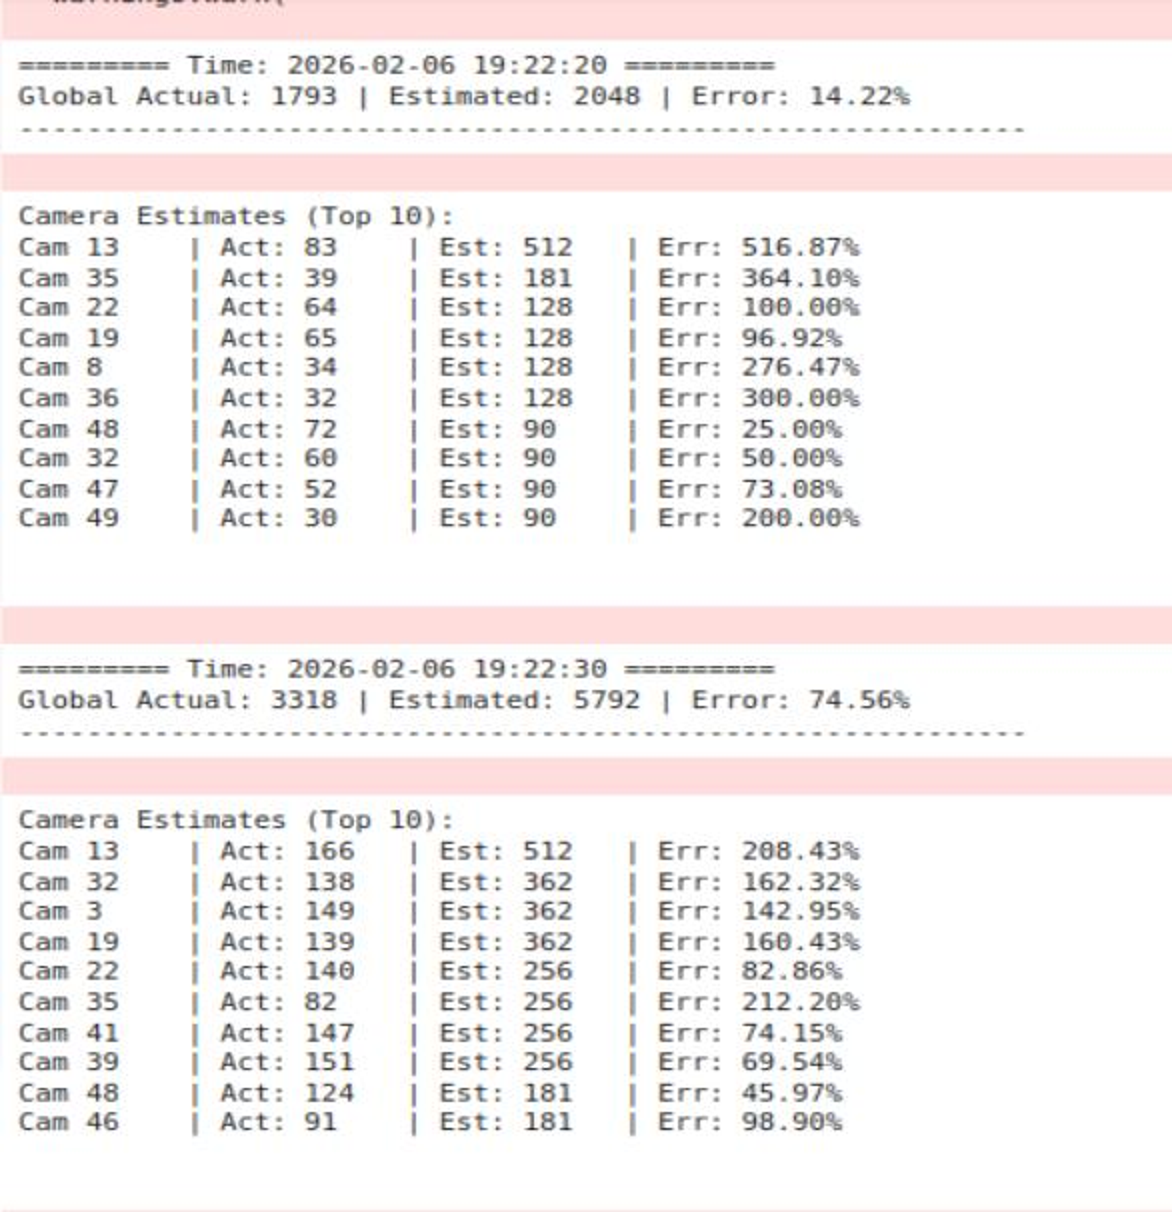
\includegraphics[width=\linewidth,height=.72\textheight,keepaspectratio]{assets/036_p034_01.png}\caption{Diagram or recorded result: Practical 2: four-hash distinct counting.}\label{fig:036_p034_010}\end{figure}
\begin{figure}[!htbp]\centering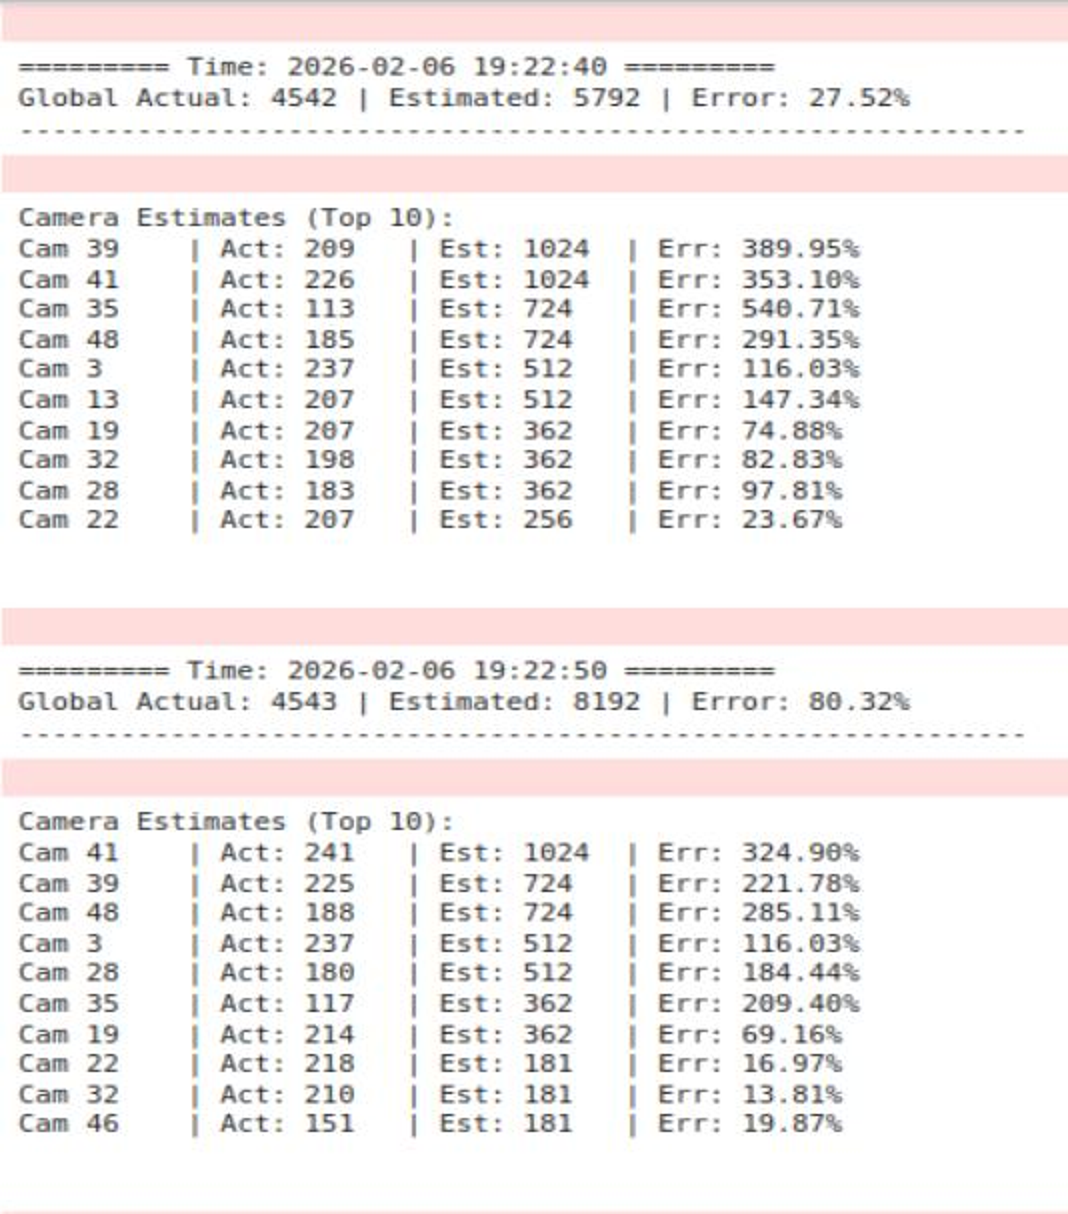
\includegraphics[width=\linewidth,height=.72\textheight,keepaspectratio]{assets/036_p034_02.png}\caption{Diagram or recorded result: Practical 2: four-hash distinct counting.}\label{fig:036_p034_020}\end{figure}
\begin{figure}[!htbp]\centering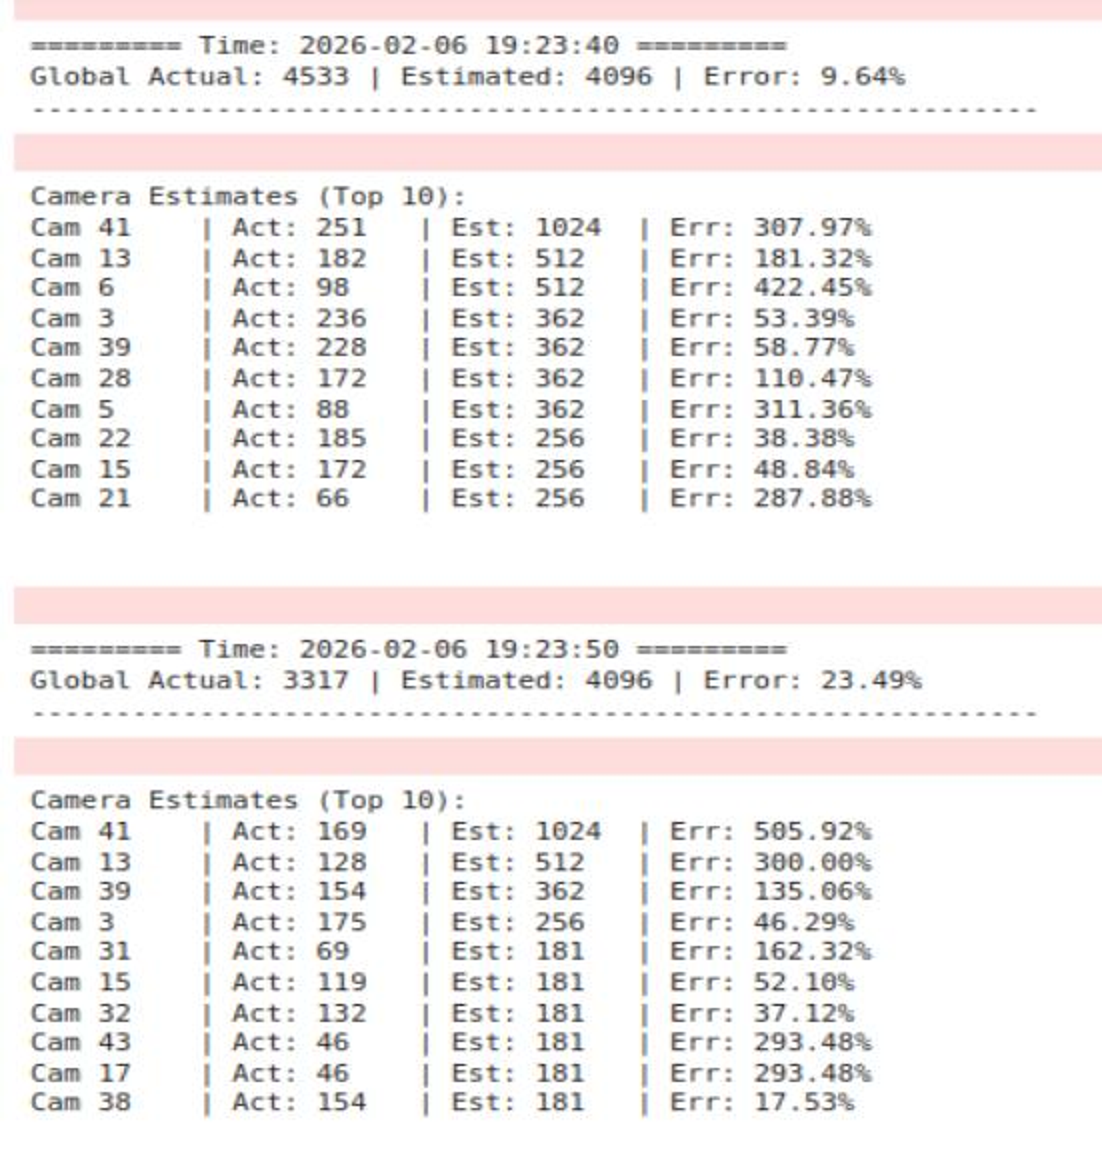
\includegraphics[width=\linewidth,height=.72\textheight,keepaspectratio]{assets/036_p034_03.png}\caption{Diagram or recorded result: Practical 2: four-hash distinct counting.}\label{fig:036_p034_030}\end{figure}
\begingroup\small\setlength{\tabcolsep}{3pt}\renewcommand{\arraystretch}{1.18}\begin{longtable}{@{}p{0.2200\linewidth}p{0.2200\linewidth}p{0.2200\linewidth}p{0.2200\linewidth}@{}}
\caption{Distinct-count estimates and absolute relative errors in two recorded windows.}\label{tab:036_p036_table10}\\\toprule
\textbf{Window} & \textbf{Actual distinct count} & \textbf{Four-register estimate} & \textbf{Absolute relative error (\%)} \\ \midrule\endfirsthead \textbf{Window} & \textbf{Actual distinct count} & \textbf{Four-register estimate} & \textbf{Absolute relative error (\%)} \\ \midrule\endhead
1 & 1730 & 2048 & 18.3815028902 \\
2 & 3318 & 2896.309375740099 & 12.7091815630 \\
\bottomrule\end{longtable}\endgroup
\clearpage
\section{Practical 3: directed camera-transition graph}

Observations are grouped by plate and sorted by recorded time. Each consecutive pair with different cameras produces an observed directed transition;\allowbreak{} repeated observations at one camera are removed as self-transitions in the described design. The report states 50 nodes and 79310 edges. For a simple directed graph with 50 nodes and no loops, at most 2450 unique directed camera pairs exist. Consequently 79310 refers to transition events or parallel edges, not unique camera-pair edges. Preserve that distinction when computing degree, weights, or drawing a simple graph. Observed transitions do not reconstruct every intervening road segment.

\begin{figure}[!htbp]\centering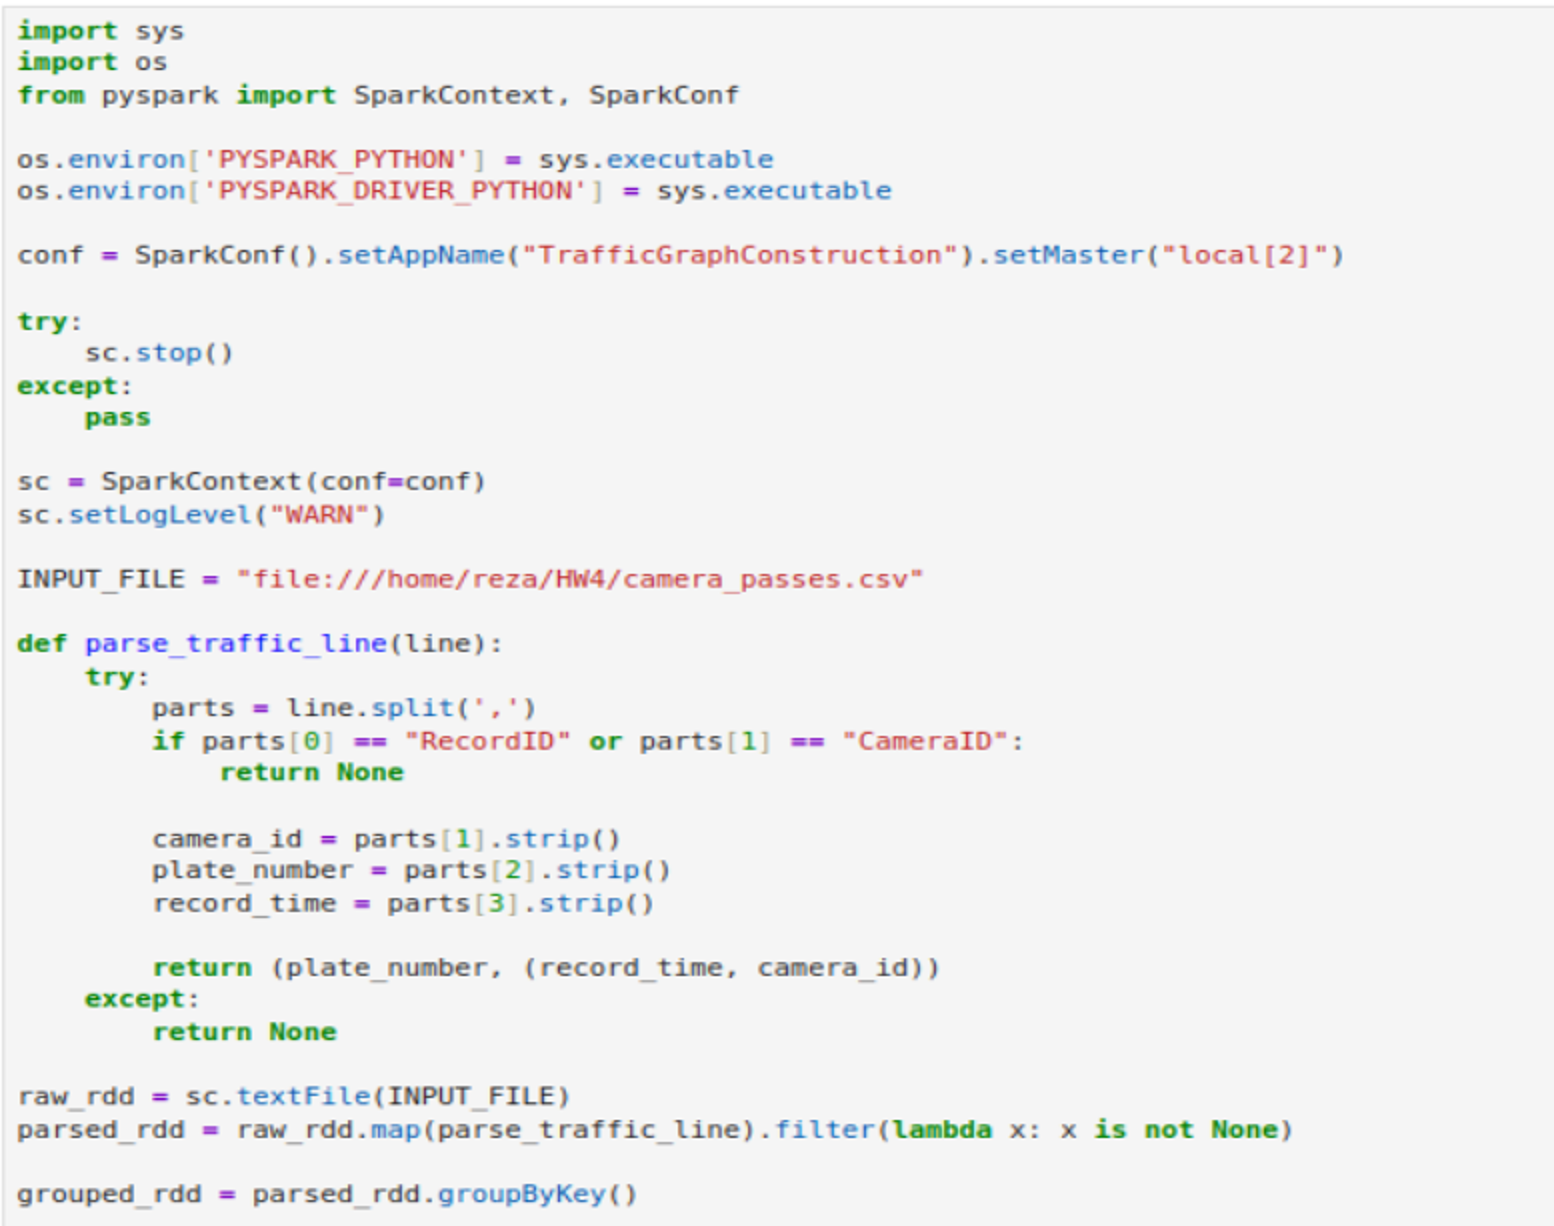
\includegraphics[width=\linewidth,height=.72\textheight,keepaspectratio]{assets/036_p038_01.png}\caption{Implementation and output: Practical 3: directed camera-transition graph.}\label{fig:036_p038_010}\end{figure}
\begin{figure}[!htbp]\centering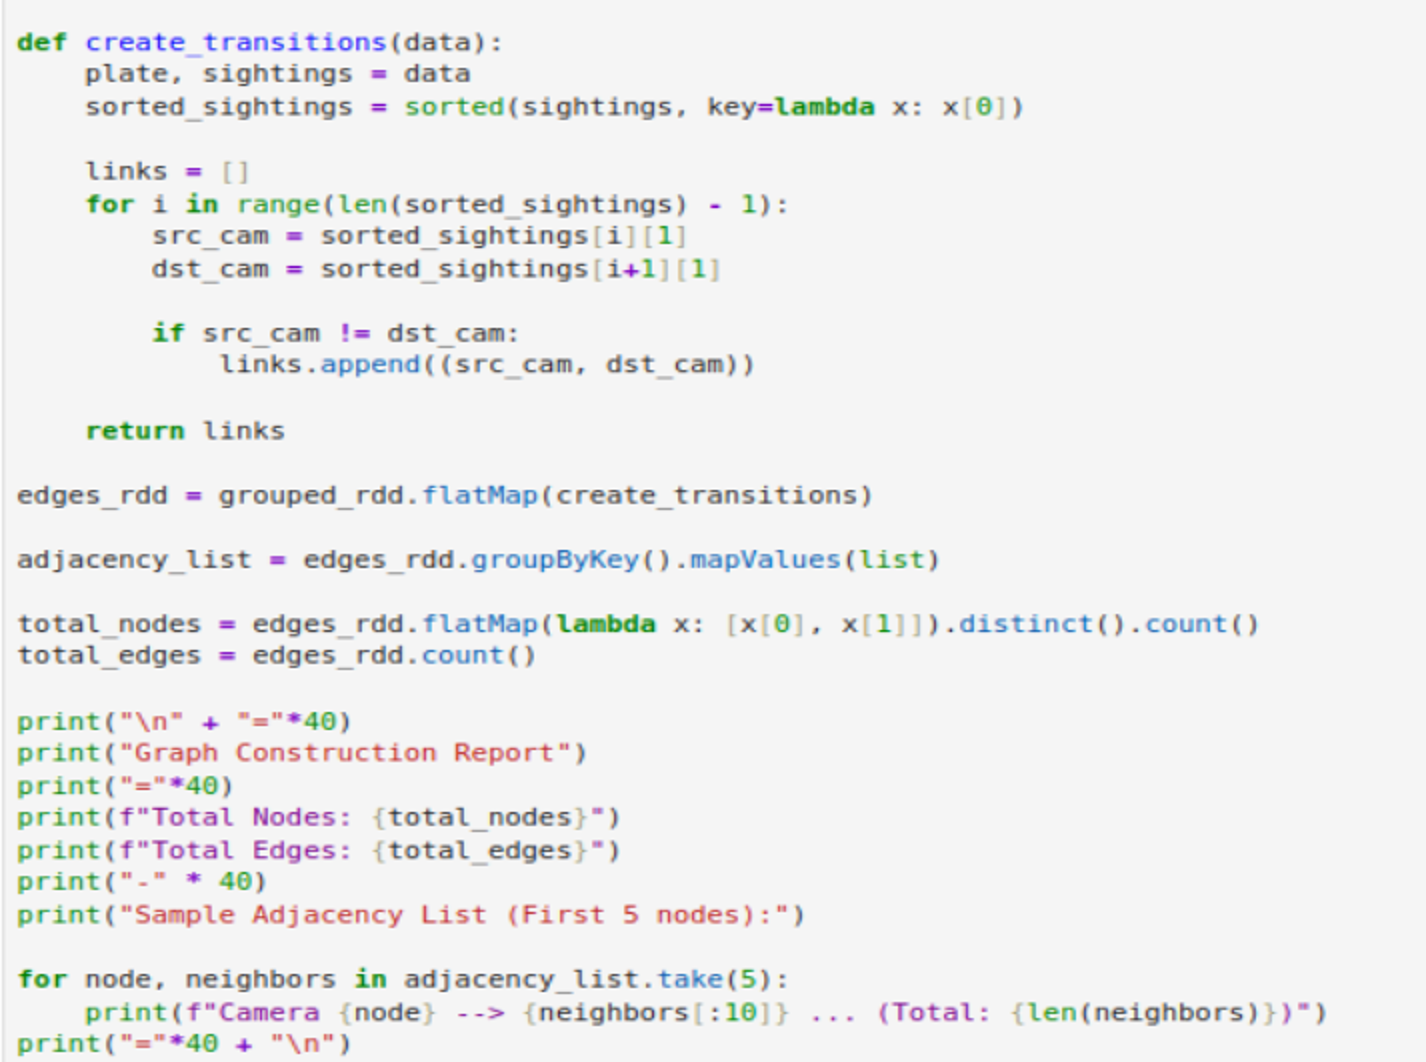
\includegraphics[width=\linewidth,height=.72\textheight,keepaspectratio]{assets/036_p038_02.png}\caption{Implementation and output: Practical 3: directed camera-transition graph.}\label{fig:036_p038_020}\end{figure}
\begin{figure}[!htbp]\centering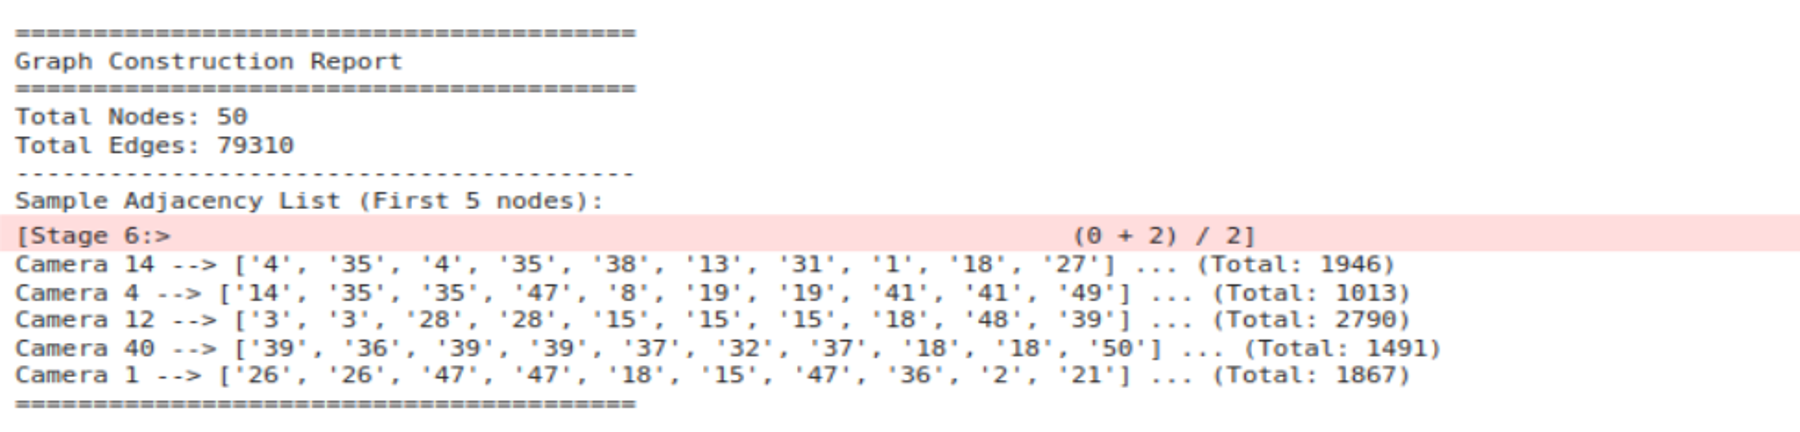
\includegraphics[width=\linewidth,height=.72\textheight,keepaspectratio]{assets/036_p039_01.png}\caption{Diagram or recorded result: Practical 3: directed camera-transition graph.}\label{fig:036_p039_010}\end{figure}
\clearpage
\section{PageRank with dangling nodes}

Ranks start at 1/\allowbreak{}N and use beta=\allowbreak{}0.85 for ten iterations. All nodes are retained through rightOuterJoin. Each iteration computes dangling mass d=\allowbreak{}sum(ranks of zero-outdegree nodes) and adds beta*d/\allowbreak{}N to every node in addition to (1-beta)/\allowbreak{}N, under uniform redistribution. For weighted transitions, normalize by outgoing weight;\allowbreak{} for an unweighted graph, normalize by outdegree. The probability-preserving recurrence is r\_\allowbreak{}new(v)=\allowbreak{}(1-beta)/\allowbreak{}N+\allowbreak{}beta*d/\allowbreak{}N+\allowbreak{}beta*sum\_\allowbreak{}u r(u)*P(u -> v). Check nonnegativity, rank sum near one, and a residual/\allowbreak{}convergence criterion. Ten iterations alone do not prove convergence. The traffic-dataset rankings are recorded outputs. The stationary four-node calculation is a separate theoretical example.

\begin{figure}[!htbp]\centering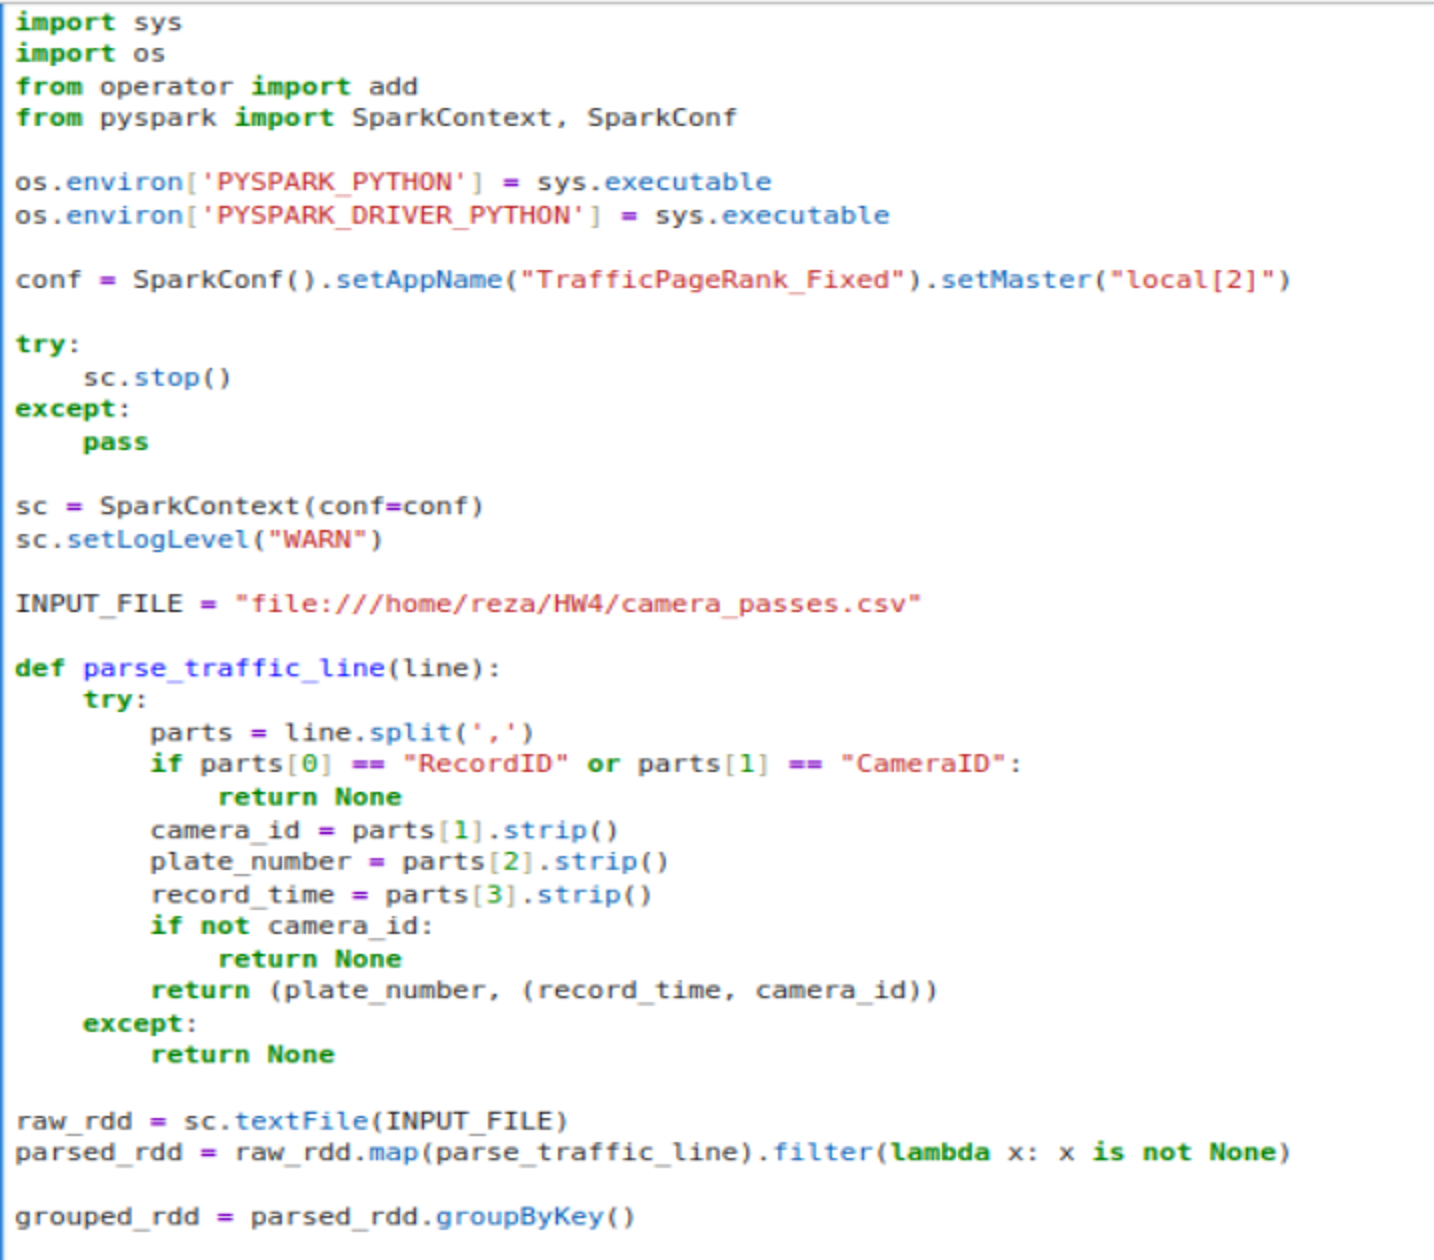
\includegraphics[width=\linewidth,height=.72\textheight,keepaspectratio]{assets/036_p040_02.png}\caption{Implementation and output: PageRank with dangling nodes.}\label{fig:036_p040_020}\end{figure}
\begin{figure}[!htbp]\centering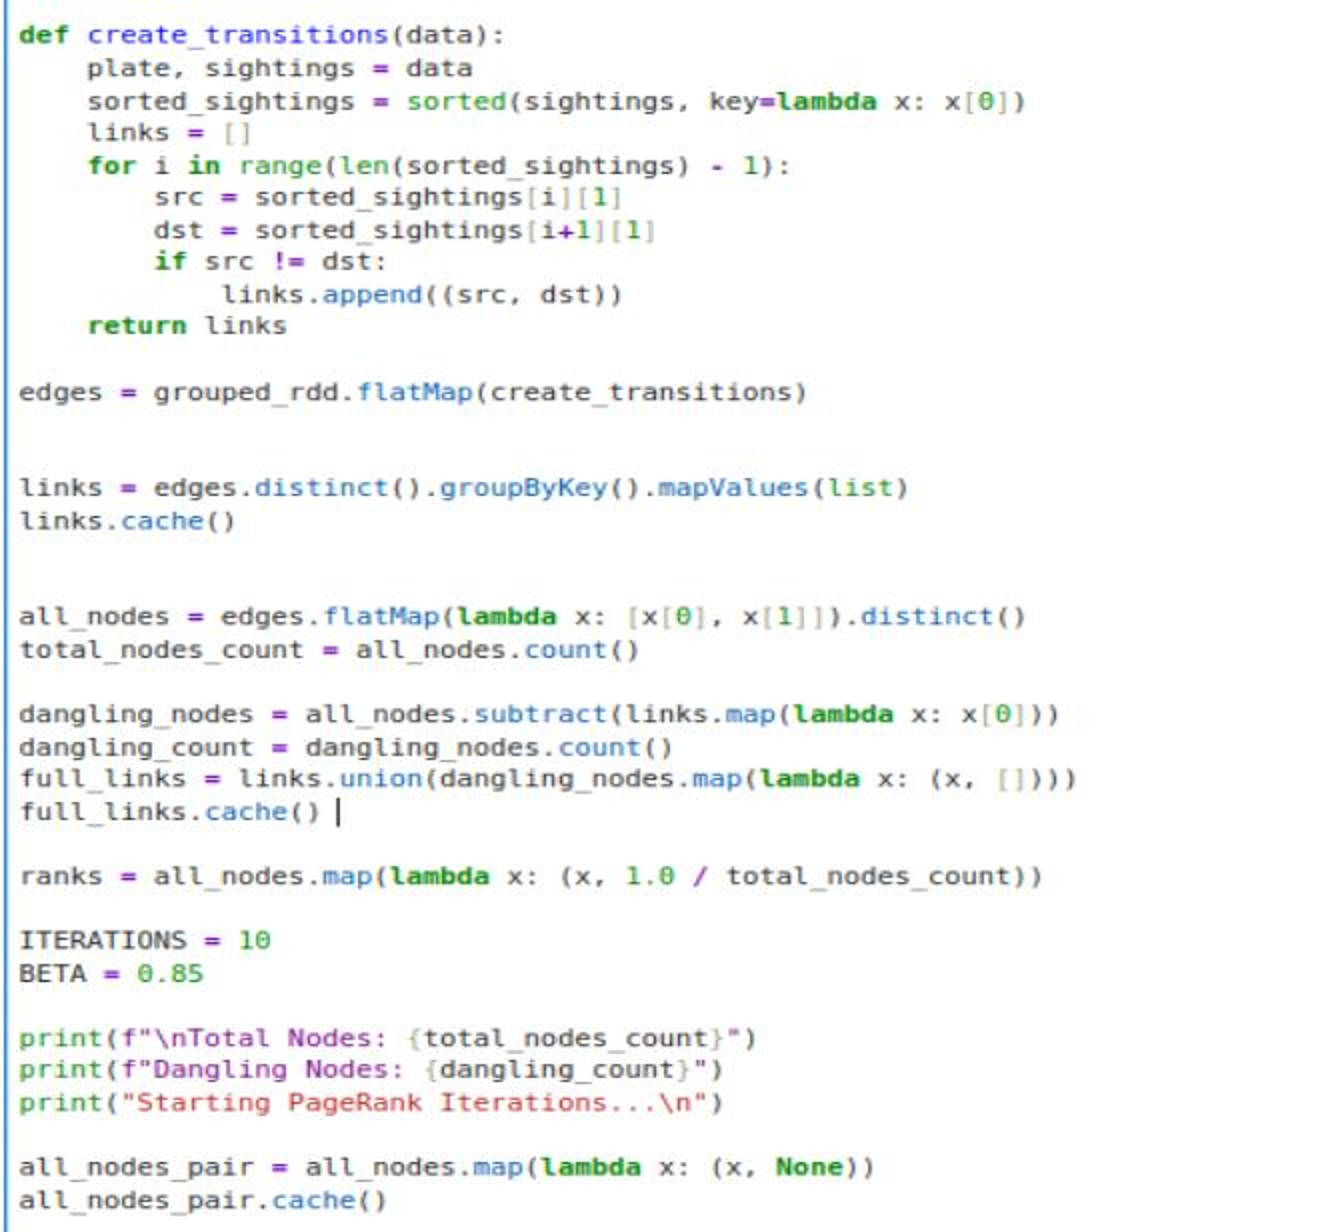
\includegraphics[width=\linewidth,height=.72\textheight,keepaspectratio]{assets/036_p040_03.png}\caption{Implementation and output: PageRank with dangling nodes.}\label{fig:036_p040_030}\end{figure}
\begin{figure}[!htbp]\centering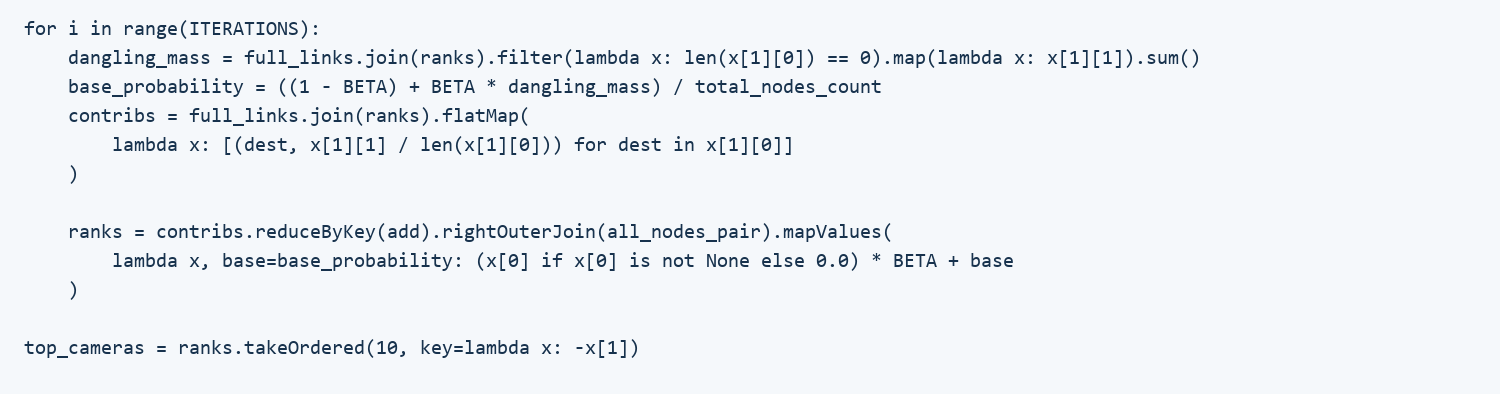
\includegraphics[width=\linewidth,height=.72\textheight,keepaspectratio]{assets/036_p040_04.png}\caption{Implementation and output: PageRank with dangling nodes.}\label{fig:036_p040_040}\end{figure}
\begin{figure}[!htbp]\centering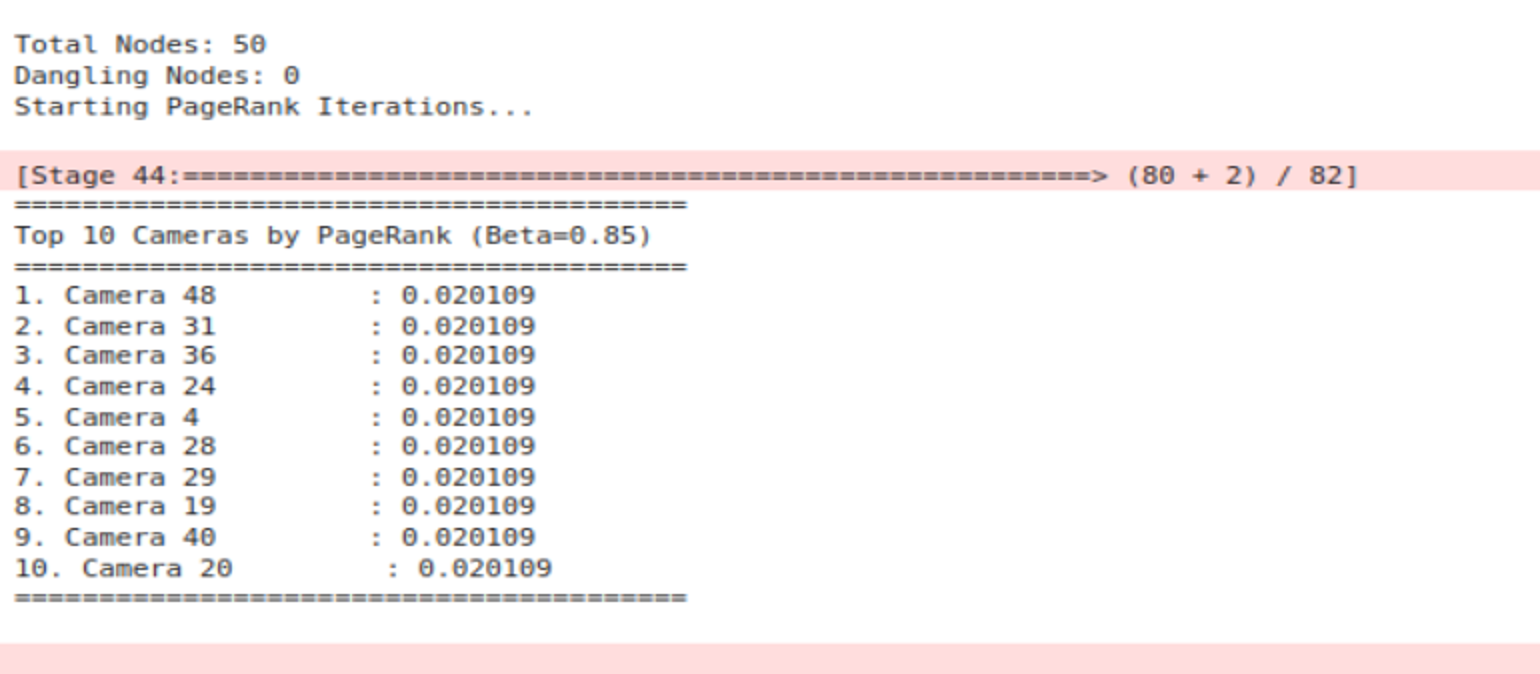
\includegraphics[width=\linewidth,height=.72\textheight,keepaspectratio]{assets/036_p041_01.png}\caption{Diagram or recorded result: PageRank with dangling nodes.}\label{fig:036_p041_010}\end{figure}
\clearpage
\section{Rankings, count comparison, and visualization}

The reported top ten are 48,31,36,24,4,28,29,19,40,20. The traffic-count top ten are 13,39,3,41,22,19,32,48,28,46. Their overlap is 48,28,19. Equal displayed ranks near 0.020109 can result from rounding, dense connectivity, or implementation choices;\allowbreak{} they do not prove structural symmetry or a main corridor.


\begingroup\small\setlength{\tabcolsep}{3pt}\renewcommand{\arraystretch}{1.2}
\begin{longtable}{@{}p{0.4775\linewidth}p{0.4775\linewidth}@{}}
\toprule
\textbf{Comparison} & \textbf{Cameras} \\ \midrule
\endfirsthead
\textbf{Comparison} & \textbf{Cameras} \\ \midrule \endhead
Both lists & 48,28,19 \\
Rank only & 31,36,24,4,29,40,20 \\
Count only & 13,39,3,41,22,32,46 \\
\bottomrule\end{longtable}\endgroup

A top-15 rank-selected subgraph is drawn with NetworkX/\allowbreak{}Matplotlib and line thickness based on transition counts. PageRank supplies a structural random-walk score, while observation totals supply volume. Neither score alone establishes a physical bottleneck, predicts disruption severity, or validates route planning. Such conclusions require topology, capacity, ground truth, and intervention evidence.

\begingroup\small\setlength{\tabcolsep}{3pt}\renewcommand{\arraystretch}{1.18}\begin{longtable}{@{}p{0.3000\linewidth}p{0.3000\linewidth}p{0.3000\linewidth}@{}}
\caption{Rankings, count comparison, and visualization - numerical data and parameters.}\label{tab:036_p044_table10}\\\toprule
\textbf{Ranking group} & \textbf{Camera identifiers} & \textbf{Interpretation} \\ \midrule\endfirsthead \textbf{Ranking group} & \textbf{Camera identifiers} & \textbf{Interpretation} \\ \midrule\endhead
High volume and high recorded rank & 19, 28, 48 & Both recorded observation volume and structural score are high \\
High recorded rank only & 31, 36, 24, 4, 29, 40, 20 & The graph-based ranking differs from simple volume \\
High volume only & 13, 39, 3, 41, 22, 32, 46 & High observed volume does not by itself imply high graph rank \\
\bottomrule\end{longtable}\endgroup
\begin{figure}[!htbp]\centering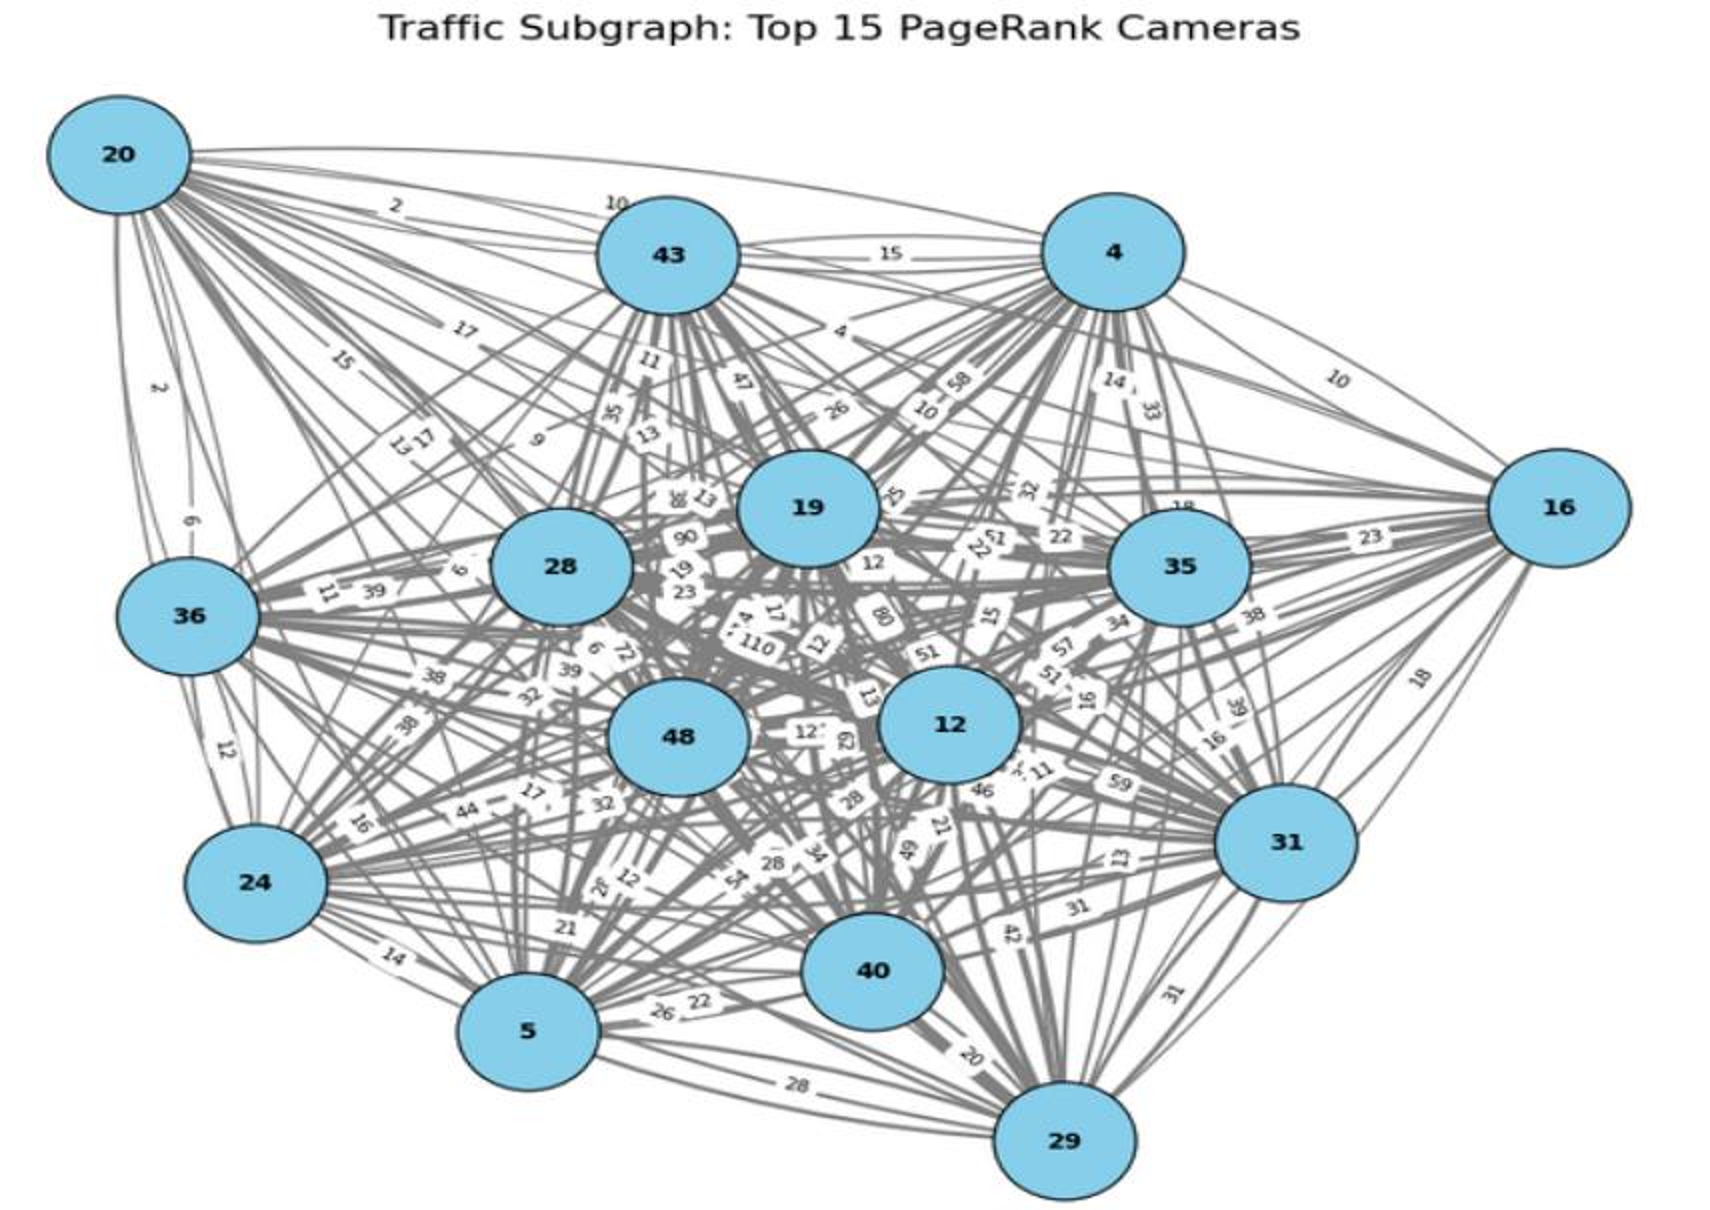
\includegraphics[width=\linewidth,height=.72\textheight,keepaspectratio]{assets/036_p046_02.png}\caption{Diagram or recorded result: Rankings, count comparison, and visualization.}\label{fig:036_p046_020}\end{figure}
\clearpage
\section{Four-node ranking results}

\begingroup\small\setlength{\tabcolsep}{3pt}\renewcommand{\arraystretch}{1.2}
\begin{longtable}{@{}p{0.1760\linewidth}p{0.1760\linewidth}p{0.1760\linewidth}p{0.1760\linewidth}p{0.1760\linewidth}@{}}
\toprule
\textbf{Model, node order A/\allowbreak{}B/\allowbreak{}C/\allowbreak{}D} & \textbf{A} & \textbf{B} & \textbf{C} & \textbf{D} \\ \midrule
\endfirsthead
\textbf{Model, node order A/\allowbreak{}B/\allowbreak{}C/\allowbreak{}D} & \textbf{A} & \textbf{B} & \textbf{C} & \textbf{D} \\ \midrule \endhead
Uniform PageRank & 0.324561404 & 0.225146199 & 0.225146199 & 0.225146199 \\
Teleport A & 0.403508772 & 0.198830409 & 0.198830409 & 0.198830409 \\
Teleport A/\allowbreak{}C & 0.373245614 & 0.183918129 & 0.258918129 & 0.183918129 \\
Trust B & 0.284903047 & 0.323453370 & 0.173453370 & 0.218190212 \\
Raw spam mass & 0.122190612 & -0.436637047 & 0.229596719 & 0.030895420 \\
HITS hubs, max normalized & 1.000000000 & 0.391943596 & 0.102775049 & 0.710831454 \\
HITS authority, max normalized & 0.289168546 & 1.000000000 & 1.000000000 & 0.813606503 \\
\bottomrule\end{longtable}\endgroup

These checks apply to the theoretical four-node graph, not a rerun of the traffic graph.

\end{document}